\documentclass[a4paper,12pt,openany]{scrreprt}
\usepackage[
	left=2.5cm, 
	right=4cm, 
    top=2.5cm, 
    bottom=2.5cm,
    footskip=10mm,
    headsep=5mm]{geometry}

\usepackage[
	pdftitle={Die Social Media Kommunikation der Universität Bielefeld und die Anwendbarkeit des Modells nach Jan-Hinrik Schmidt},
    pdfsubject={Bachelorarbeit im Kernfach Linguistik - Universität Bielefeld},
    pdfauthor={Fabian Wohlgemuth},
    pdfkeywords={BA, Bachelorarbeit, Bachelor thesis, Social Web, Social Media, Kommunikation, Universität Bielefeld},
    %pdftex=true,
    colorlinks=true,
    citecolor=black,
    linkcolor=black,
    menucolor=black,
    urlcolor=black
]{hyperref}

\usepackage[utf8]{inputenc}
\usepackage[T1]{fontenc}
\usepackage{graphicx}
\usepackage{graphicx, subfigure}
\graphicspath{{images/}}
%\usepackage{fancyhdr}
\usepackage{lmodern}
\usepackage{color}
\usepackage[table, dvipsnames]{xcolor}

\usepackage{transparent}
\usepackage[ngerman]{babel}

\usepackage{lipsum}

\usepackage{datetime2}

\usepackage{setspace}
\onehalfspacing

\usepackage{tikz}

\usepackage{float}

\usepackage{amsmath}
\usepackage{amsfonts}
\usepackage{calc}

\usepackage{subfig}

\usepackage{csquotes}
\MakeOuterQuote{"} 

%%%
\input{pgfutil-common.tex}
\usepackage{pgfkeys,pgfmath}  
\usepackage{siunitx}

\newcommand{\printpercent}[3][2]{%  
    \pgfmathdivide{#2}{#3}% 
    \pgfmathmultiply{\pgfmathresult}{100}%
    \SI[round-mode=places,round-precision=#1]{\pgfmathresult}{\percent}
}
%%%

\usepackage{acronym}

\usepackage{fontawesome}

\usepackage[nottoc,notlot,notlof]{tocbibind}

% \setlength{\parindent}{0pt}

%\pagestyle{fancy}
%\fancyhead{}
%\fancyfoot{}
%\fancyfoot[R]{\thepage}

\begin{document}

\pagestyle{empty}
\newgeometry{left=1.5cm,right=1.5cm,top=2cm,bottom=2cm}
\begin{center}

\Huge{\textbf{Universität Bielefeld}}

\LARGE{Fakultät für Linguistik und Literaturwissenschaft}

\vfill

\LARGE{\textbf{Bachelorarbeit}}

\Large

im Kernfach Linguistik

\vfill

zum Thema:

\vspace*{1cm}

\LARGE{\textbf{Die Social Media Kommunikation der Universität Bielefeld und die Anwendbarkeit des Modells nach Jan-Hinrik Schmidt}}

\Large

\vfill

vorgelegt von

\vspace*{1cm}

\textbf{\href{https://www.fabianwohlgemuth.de}{Fabian Wohlgemuth}}

\vfill

$\begin{aligned}
\text{Erstgutachterin:}&\ \text{Frau Dr. Petra Pansegrau}\\
\text{Zweitgutachterin:}&\ \text{Frau Prof. Dr. Barbara Job}
\end{aligned}$

\vfill

Bielefeld, im September 2018

\end{center}
\restoregeometry

\pagenumbering{Roman}

%\addcontentsline{toc}{section}{Danksagung}\setcounter{page}{2}\chapter*{Danksagung}
\label{chap:Danksagung}

danke
%\addcontentsline{toc}{section}{Abstract}\chapter*{Abstract}
\label{chap:Abstract}

\section*{figure}
\begin{figure}[h]
figure example
\caption{nice figure}
\label{fig: nice figure}
\end{figure}

\section*{table}
\begin{table}[h]
\begin{tabular}{ l c r}
4 & 4 & 4 \\
\hline \\
5 & 5 & 5 
\end{tabular}
\caption{table table table}
\label{tab:table table table}
\end{table}
\addcontentsline{toc}{section}{Inhaltsverzeichnis}
\newpage

\tableofcontents

\newpage
\let\LaTeXStandardClearpage\clearpage
\let\clearpage\relax

\begin{spacing}{1.1}
\addcontentsline{toc}{section}{Abbildungs-, Tabellenverzeichnis}\listoffigures \listoftables
%\chapter*{Abkürzungsverzeichnis}
\label{chap:Abkürzungen}

\begin{acronym}[Bash]
 \acro{SMK}{Social Media Kommunikation}
 \acro{SMP}{Social Media Plattform}
 \acro{Uni Bielefeld}{Universität Bielefeld}
\end{acronym}
\end{spacing}

\addtocontents{toc}{\vspace{\normalbaselineskip}}
\addtocontents{toc}{\hrule}
\addtocontents{toc}{\vspace{\normalbaselineskip}}
\let\clearpage\LaTeXStandardClearpage
\newpage
\pagenumbering{arabic}

\newpage
\chapter{Einleitung}
\label{chap:Einleitung}

% Zielsetzung - Problemstellung - Eingrenzung/Abgrenzung des Themas (begründet) - Aufbau - Roter Faden

Diese Abschlussarbeit widmet sich dem immer relevanter werdenden Thema der Social Media Kommunikation. Unter anderem durch Jan-Hinrik Schmidt, gibt es im deutschsprachigen Raum ein sehr aktives Forschungsfeld um die Thematiken des Social Web. Viele der Forschungsansätze untersuchen jedoch in erster Linie die Social Media Kommunikation im Rahmen der Nutzung durch Einzelpersonen.

Mit der steigenden Relevanz der sozialen Medien auch für Firmen und Institutionen, für die inzwischen das Social Media Marketing auch nicht mehr wegzudenken ist, beschäftigen sich jedoch im Verhältnis eher wenige Forschungsarbeiten.

In der heutigen Zeit, und zum laufenden Beginn der Digitalisierung, ist ein Blick auf gebräuchliche Kommunikationsmodelle angebracht, die sich, wie der Großteil der Forschung, der Kommunikation unter Personen widmet, um festzustellen, ob diese auch Anwendbarkeit finden, in der Kommunikation zwischen Firmen, Institutionen und anderen Einrichtungen, und deren Social Media Followern.

Im Speziellen möchte ich mir das Kommunikationsmodell nach Jan-Hinrik Schmidt anschauen, welches, mit den Begriffen \textit{Identitätsmanagement}, \textit{Beziehungsmanagement} und \textit{Informationsmanagement}, die Social Media Kommunikation von Einzelpersonen zu klassifizieren versucht. Dieses Modell soll im Laufe dieser Arbeit auf die Anwendbarkeit auf die Social Media Kommunikation der Universität Bielefeld -- als Beispiel einer Institution -- untersucht werden. \smallskip

Anfangen werde ich in Kapitel \ref{chap:Theorie} mit dem theoretischen Hintergrund, einer kurzen geschichtlichen Einleitung, und der Beschreibung der meist genutzten Social Media Plattformen -- sowohl allgemein als auch innerhalb der Social Media Kommunikation der Universität Bielefeld. Danach werde ich den aktuellen Stand der Forschung in Kapitel \ref{sec:aktuelleforschung} skizzieren, und mit Hilfe dessen, über begründete Forschungsfragen, zu den Hypothesen dieser Arbeit in Kapitel \ref{sec:hypothesen} überleiten.

Anschließend folgt in Kapitel \ref{chap:Empirie} die empirische Verarbeitung. Dort werde ich die genutzten Daten beschreiben und sie auf der Forschungsgrundlage aus Kapitel \ref{sec:jhsforschung} verarbeiten. Die Ergebnisse der Verarbeitung stelle ich dann in Kapitel \ref{sec:Ergebnisse} vor, und werde sie anschließend in Kapitel \ref{sec:Diskussion} analysieren und diskutieren.

Den Schluss bilden in Kapitel \ref{chap:Fazit} das Fazit meiner Analysen, die kritische Betrachtung der Herangehensweise dieser Arbeit, und ein Ausblick auf weiter zu untersuchende Forschungsfragen.

% Ziel der Arbeit ist es, das untersuchte Kommunikationsmodell zu erweitern oder zu verändern, um sich dem entwickelten Anspruch anzupassen, und die Social Media Kommunikation von Institutionen in dem Modell unterbringen zu können.

\chapter{Theoretischer Hintergrund}
\label{chap:Theorie}
\pagestyle{plain}

Zu Beginn dieser Arbeit werde ich eine kurze Einführung in die Geschichte des Internets, und den in ihm immer größer werdenden Anteil der sozialen Medien geben. Auf letztere werde ich dann im Detail eingehen, indem ich die gängigsten Social Media Plattformen beschreibe und dann eine Übersicht der zugänglichen Plattformen gebe. Im Anschluss werde ich auf die Plattformen eingehen, die die Universität Bielefeld sich zu Nutze macht.

\section{Das Internet und die sozialen Medien}

Als Tim Berners-Lee Ende der 80er Jahre mit der Entwicklung des World Wide Web den Wissenschaftlerinnen und Wissenschaftlern des CERN in der Schweiz einen Gefallen tun, und den Austausch von Daten und Informationen innerhalb der Einrichtung für Kernforschung vereinfachen wollte \cite{w3cpeople}, hatte er sicherlich nicht das Ausmaß im Kopf, welches das Internet, so wie wir es heute kennen, annehmen, und ihm im Jahre 2004, 24 Jahre nach Beginn seiner Internet-Karriere, für seine Dienste an der globalen Entwicklung des Internets die Ritterwürde bringen sollte \cite{w3cbernerslee}. Berners-Lees Arbeit waren schon knapp zwei Jahrzehnte der Entwicklung vorangegangen, in denen über das ARPANET, welches Ende der 60er Jahre erste Gestalt annahm, am Beginn der 70er Jahre die erste Mail versendet werden konnte \cite{gillies2000web}.

Die rapide Entwicklung der Internet-Techniken begünstigt seit vielen Jahren den Informationsaustausch und die Möglichkeit zur individuellen und Gruppen-Kommunikation und vereinfacht diese stets weiter. So sind die Dienste des Internets schon lange nicht mehr ein Privileg von Forschungseinrichtungen wie dem CERN, Universitäten, oder militärischen Einrichtungen. Über 50 Prozent der Erdpopulation hat bereits regelmäßigen Internetzugang, wie eine statista-Studie von Juli diesen Jahres zeigt \cite{statista2018digpop}. Eine solch hohe Zahl ist auch der Entwicklung der sozialen Medien zu verdanken, wie man den Nutzungsstatistiken der großen Social Media Plattformen entnehmen kann, auf die später in diesem Kapitel noch eingegangen wird.

Die Nutzung des Internets, und den in ihrer Popularität immer weiter steigenden Social Media Plattformen, die "[...] einen neuartigen Raum zwischen massenmedialen und der interpersonalen Kommunikation schaffen und einnehmen"\  \cite{schmidt2018einstieg}, ist aus dem Alltag der meisten Menschen überhaupt nicht mehr wegzudenken. Doch was gehört zu diesen Social Media Plattformen dazu? Warum ist eine Internetnutzung ohne Social Media Plattformen heutzutage nicht mehr denkbar? Im Folgenden möchte ich eine Übersicht über bekannte Social Media Plattformen geben, um diesen Fragen nachzugehen.

\subsection{Social Media Plattformen}

\subsubsection{Facebook}

Die wohl bekannteste und meist genutzte Social Media Plattform ist Facebook \faFacebook. Mit täglich ca. 1,4 Milliarden Nutzerinnen und Nutzern \cite{facebookfinancials} nutzten laut des eigenen Firmenreports im Dezember 2017 jeden Tag ein knappes Fünftel der gesamten Menschheit, also ein knappes Drittel der aktiven Internetnutzer, Facebook. Facebook kombiniert viele Gesichtspunkte der sozialen Kommunikation und Interaktion in einer Oberfläche, was eine vielfältige Nutzung ermöglicht. Angefangen mit klassischer Eins-zu-eins-Kommunikation im privaten Chat, über private Gruppenkommunikation bis hin zu öffentlichen Diskussionsmöglichkeiten in wiederum geschlossenen oder öffentlichen Interessensgemeinschaften, bietet Facebook seinen Nutzerinnen und Nutzern das gesamte Spektrum der sozialen Kommunikation. Über die direkte Kommunikation hinaus, ist die indirekte Kommunikation zur Außenwelt --ob einer eingeschränkt privaten, oder aber auch der gesamten, öffentlich zugänglichen-- ein großer Teil der Social Media Plattform und gleichzeitig auch der Bildung von persönlichen Öffentlichkeiten, einem "[...] Geflecht von online zugänglichen kommunikativen Äußerungen zu Themen von vorwiegend persönlicher Relevanz [...]"\ \cite{schmidt2009netz}.

Auf Facebook ist es der Nutzerin und dem Nutzer möglich, sowohl Text- als auch Bild- und Video-Beiträge zu erstellen, oder aber auf im Internet schon vorhandene Information zu verlinken. Dabei kann die sogenannte Timeline, also die chronologische Gesamtheit der Beiträge einer Nutzerin oder eines Nutzers, zur Informationsweitergabe, zur Dokumentation eigenen Wissens oder eigener Erlebnisse, oder aber auch zum Aufbau oder zum Erhalt von Beziehungen dienen.

Zusätzlich zu dieser Produzenten-Funktion kommt bei den meisten Social Media Plattformen --auch bei Facebook-- die Funktion des Rezipienten hinzu. Die Nutzerin und der Nutzer der Plattform Facebook kann nicht nur eigene Inhalte teilen sondern gibt mit der Veröffentlichung eigener Informationen und Beiträge auch anderen Nutzerinnen und Nutzern die Möglichkeit, auf Beiträge zu reagieren und/oder zu kommentieren und auch die Beiträge weiter auf der eigenen Timeline oder in anderen Gruppen/Interessensgemeinschaften zu teilen.

\subsubsection{Weblogs}

Weblogs, im weiteren Verlauf verkürzt Blogs, sind eine digitale Form des Tagebuchs. Der Begriff setzt sich aus den Teilen \textit{Web} und \textit{Log(buch)} zusammen. Der Unterschied zwischen einer Social Media Plattform wie Facebook, und dem klassischen Blog, ist die Funktion der/des Blogführenden. Diese/r nimmt in erster Linie nur die Rolle des Produzenten ein, da es sich beim klassischen Blog um die Herausgabe von Informationen und Wissen von einer stärker als bei anderen Social Media Plattformen eingeschränkten Personengruppe handelt. So werden einige der bekanntesten Blogs von Einzelpersonen geführt\footnote{Beispiele im deutschsprachigen Raum:\\Fefes Blog, \url{https://blog.fefe.de/}; Technikfaultier, \url{https://www.technikfaultier.com}}; einige andere wiederum von kleinen Personengruppen. Auch Firmen und Institutionen machen sich mittlerweile Blogsysteme zu nutze, um in klassischer Zeitungsmanier regelmäßig Informationen zu verbreiten.

In den meisten Blogsystemen sind mittlerweile Kommentarfunktionen eingebaut, die mehr oder minder häufig von den Betreibenden auch genutzt werden. Da es sich hierbei jedoch nicht unbedingt um einen Kernbaustein des Systems handelt, ist dieser Funktions-Unterschied zu anderen Social Media Plattformen entscheidend.

Zu den am häufigsten genutzten Blog-Plattformen gehören WordPress \faWordpress, Googles Blogger und Medium \faMedium.

\subsubsection{Twitter}

Twitter \faTwitter\ ist der populärste Vertreter der Blog-Unterkategorie Mikroblog. Ein besonderes Merkmal der Plattform ist, dass Beiträge in Ihrer Länge stark limitiert sind. Angefangen bei nur 140 Zeichen, ist die Begrenzung mittlerweile auf 280 Zeichen angehoben worden. Dennoch bleibt Twitter eine der wenigen populären Mikroblog-Plattformen.

Ein Tweet, also ein Beitrag auf Twitter, kann innerhalb der 280 Zeichen normalen Text, aber auch Bilder und Kurzvideos und Links zu anderen Webseiten oder Medien darstellen. Die Besonderheit dabei ist die Möglichkeit zum einen, einen Tweet mit Schlagworten, sogenannten \textit{Hashtags} zu versehen, indem dem gewünschten Schlagwort ein \# vorangestellt wird, und zum anderen die Möglichkeit, andere Nutzerinnen und Nutzer der Plattform direkt zu adressieren, indem dem Nutzernamen der zu kontaktierenden Person ein @ vorangestellt wird. Der Tweet \textit{"@wohfab recherchiert zum Thema \#socialmedia."} würde also den Autor dieser Abschlussarbeit direkt adressieren und ihn über den Tweet benachrichtigen, und jeder Nutzerin und jedem Nutzer die Möglichkeit geben, nach dem Schlagwort \textit{\#socialmedia} zu suchen, und andere Beiträge mit gleichem Schlagwort zu finden und zu lesen. Beide sogenannten Tags, also sowohl die Hashtags als auch die Namenstags, werden bei Twitter automatisch zu anklickbaren Links.

Die Tweets können dann von anderen Nutzerinnen und Nutzern mit einem Herz markiert, kommentiert, und in der eigenen Twitter-Historie geteilt werden. Letzteren Vorgang wird innerhalb der Plattform als Retweeten -- also \textit{nochmal Tweeten} -- bezeichnet.

\subsubsection{Instagram}

Als Tochterfirma von Facebook \cite{instagramtou}, hat sich Instagram \faInstagram\ auf die Nutzung auf mobilen Endgeräten, und auf visuelle Medien spezialisiert. Angefangen mit Bildern, können mittlerweile auch Videos in normalen Beiträgen und sogenannten Stories geteilt werden. Letztere sind in einem zeitlich begrenzten Rahmen sichtbar und werden danach für die Öffentlichkeit unzugänglich gemacht. In Abgrenzung zu einem klassischen Blog, sind Beiträge auf Instagram --insbesondere die Story-Beiträge-- also eher kurzlebig.

Wie Twitter --und mittlerweile auch Facebook-- setzt Instagram stark auf die Nutzung von Hash- und Namenstags zur Kategorisierung und Adressierung von Beiträgen. Gegenüber Twitter hat Instagram den Vorteil, dass die Beiträge in Ihrer Länge nicht stark limitiert sind. Ein Instagram-Beitrag kann also sehr umfangreich kommentiert und zusätzlich mit einer großen Menge an Schlagworten ausgezeichnet werden. Besonders um über den eigenen Nutzerkreis hinaus Bekanntheit zu erlangen, werden für Instagram-Beiträge eine Vielzahl an Schlagworten genutzt, die sich auch wie die Timelines von Nutzerinnen und Nutzern abonnieren lassen.

\subsubsection{Snapchat}

Eine ebenfalls auf Bild- und Videomaterial spezialisierte Social Media Plattform ist Snapchat \faSnapchat. In Abgrenzung zu Instagram basiert Snapchat vollständig auf der Kurzlebigkeit seiner Beiträge, die nach geringem Zeitfenster grundsätzlich der Öffentlichkeit unzugänglich gemacht werden. Trotz der sehr speziellen Art dieser Plattform, begeistern sich jedoch täglich mehr Nutzerinnen und Nutzer an Snapchat.

\subsubsection{Karriere-Plattformen - LinkedIn und XING}

Mit LinkedIn \faLinkedin\ und XING \faXing\ sind wir mittlerweile bei den eher untypischen Social Media Plattformen angekommen. Diese beiden Plattformen können der Kategorie Karriere-Plattform zugeordnet werden. Sie dienen der Vernetzung innerhalb der Berufswelt. XING beschränkt sich dabei sehr auf den deutschsprachigen Raum; LinkedIn wird international genutzt. Ansonsten unterscheiden sich die beiden Plattformen nur in wenigen Details.

Auf solchen Karriere-Plattformen lässt sich ein Profil anlegen, auf dem der schulische und berufliche Werdegang, abgeschlossene Schulungen und erhaltene Zertifikate, besonderes Wissen und besondere Fähigkeiten und Karriere- und Forschungsinteressen mit der Öffentlichkeit oder bestimmten Personenkreisen geteilt werden können. 

\subsubsection{WhatsApp, Telegram und co.}

Auch sogenannte Instant Messaging Dienste, deren Kernfunktion die Direktkommunikation zwischen zwei Nutzerinnen/Nutzern ist, zählen zu den Social Media Plattformen. SMS und MMS aus früheren Jahren sind in unseren Breitengraden mittlerweile von Diensten wie WhatsApp \faWhatsapp, Telegram und co. abgelöst worden. Der Messaging Dienst von Facebook gehört ebenfalls zu diesen Instant Messaging Diensten. Lange Zeit war dieser an einen Facebook-Account geknüpft. Inzwischen kann man den Facebook Messenger mit einer Telefonnummer und unabhängig von einem Facebook-Account nutzen. iMessages \faApple\ ist ein Apple-Exklusiver Instant Messaging Dienst, der im Apple-Ecosystem große Beliebtheit erlangt hat; dessen größter Nachteil jedoch die System-Exklusivität ist. WhatsApp hat laut eigener Angabe im firmenblog über eine Milliarde aktive Nutzer täglich \cite{whatsappblog} und ist somit der meistgenutzte Instant Messaging Dienst weltweit.

\subsubsection{Audio- und Video-Telefonie mit Skype und Discord}

So wie Skype \faSkype, gehört auch Discord zu den Audio- und Video-Chat-Plattformen. Skype gehörte lange zur Standardplattform für Video-Telefonie und wird auch heutzutage im Enterprise-Bereich noch häufig genutzt. Discord kam vor nicht allzu langer Zeit auf diesem Markt hinzu und startete als Kommunikationsplattform für Videospielende. Die Simplizität, der Funktionsumfang der Applikationen und sowohl die Audio- als auch die Video-Qualität der Plattform haben Skype jedoch in vielen Fällen überholt und für viele Nutzerinnen und Nutzer ersetzt.

Als weitere Audio-Kommunikations-Plattformen sind noch TeamSpeak und Mumble zu nennen, die ebenfalls im Videospiel-Klientel ihre Ursprünge haben; jedoch wie Skype auch in vielen Fällen durch Discord abgelöst wurden.

\subsubsection{Wikis als moderne Variante des Forums}

Ebenfalls eher untypische Social Media Plattformen sind sogenannte Wikis. Sammlungen von Wissen, sogenannte Knowledge Bases, wie die Online-Enzyklopädie Wikipedia, setzen auf die Zusammenarbeit der Nutzerinnen und Nutzer, um die Gesamtheit des Weltwissens zu archivieren. Die Wikipedia \faWikipediaW\ ist mit Sicherheit die größte öffentlich zugängliche Knowledge Base und bekommt nach eigenen Angaben alleine auf der deutschen Variante im Durchschnitt über 32 Millionen Aufrufe pro Tag \cite{wikipediastatistik}. Neben der Wikipedia gibt es eine schier unendliche Masse an Wikis, die sich mit zum Teil sehr spezifischen, eingeschränkten Themenbereichen auseinandersetzen und häufig eine moderne Variante eines Forums darstellen, was in den Anfängen der Social Media Plattformen eine sehr übliche Art der Wissenserhaltung und der sozialen Kommunikation war.

\subsubsection{Reddit, die Startseite des Internets}

Ebenfalls Ähnlichkeiten zum klassischen Forum, weist Reddit \faReddit\ auf. Reddit kann als Meta-Forum bezeichnet werden. Es ist in mittlerweile ca. 1,2 Millionen Unter-Foren, sogenannte Subreddits aufgeteilt \cite{redditmetrics}, die sich jeweils unterschiedlichen Thematiken widmen. Diese Subreddits reichen von Nachrichten-Seiten, über Fan-Seiten für Film \& Fernsehen, bis hin zu Spaß-Seiten, die dem reinen Vergnügen dienen.

\subsubsection{Weitere Plattformen}

Neben den oben genannten Plattformen existiert eine große Menge an weiteren Plattformen, von denen ich einige bekannte Vertreter zumindest erwähnen und kategorisieren möchte.

\textbf{Video} -- YouTube \faYoutube\ und Vimeo \faVimeo\ gehören beispielsweise zu den Video-Plattformen. Die Kernfunktionalität der Plattformen ist das Veröffentlichen von fertigen Videos. Im Gegensatz dazu, setzt zum Beispiel Twitch auf die Funktionalität des Streamings. Videos werden also live übertragen, statt sie zu bearbeiten und zu schneiden, um sie dann im fertigen Format hochzuladen. Twitch ist sehr beliebt im Gaming-Bereich.

\textbf{Foto} -- Flickr \faFlickr\ , Behance \faBehance\ , 500px \faicon{500px}, Deviantart \faDeviantart\ sind Vertreter der Foto-Plattformen. Behance hat zusätzlich zum Teilen selbst erstellter Fotos einen besonderen Fokus auf Grafikdesign und die Monetarisierung desselben. Deviantart ist eine Indie-Grafiker-Plattform, die zu großen Teilen für sogenannte Fanarts verwendet wird.

\textbf{Audio} -- Die wohl bekannteste soziale Audio-Plattform ist Soundcloud \faSoundcloud. Nicht nur Künstlerinnen und Künstler können hier Ihre Werke veröffentlichen und mit ihren Fans über Kommentare und Reaktionen auf die hochgeladenen Stücke in Kontakt kommen. Soundcloud bietet eine Plattform für jegliche Art von Audiomaterial.

\textbf{Chat} -- IRC, Internet Relay Chat, wird oft mit Computerspezialistinnen und -spezialisten, meist auch mit Hackern in Verbindung gebracht. Das rein textbasierte Chatsystem läuft ohne viel Aufwand und ohne viel Ressourcen auf nahezu jedem Server und bietet somit für die Kommunikation über reinen Text eine praktische Plattform. IRC ist organisiert in Server und innerhalb dieser in sogenannte Channels, die sich zur besseren Übersicht in bestimmte Themenbereiche einteilen.

\subsubsection{Übersicht}

Alleine die Zusammenfassungen der oben genannten, bekanntesten Social Media Plattformen ist sehr umfangreich, was einen Hinweis auf die Masse an Plattformen geben kann, die in ständiger Benutzung sind und sich täglich weiterentwickeln.

\begin{figure}[h]
    \centering
    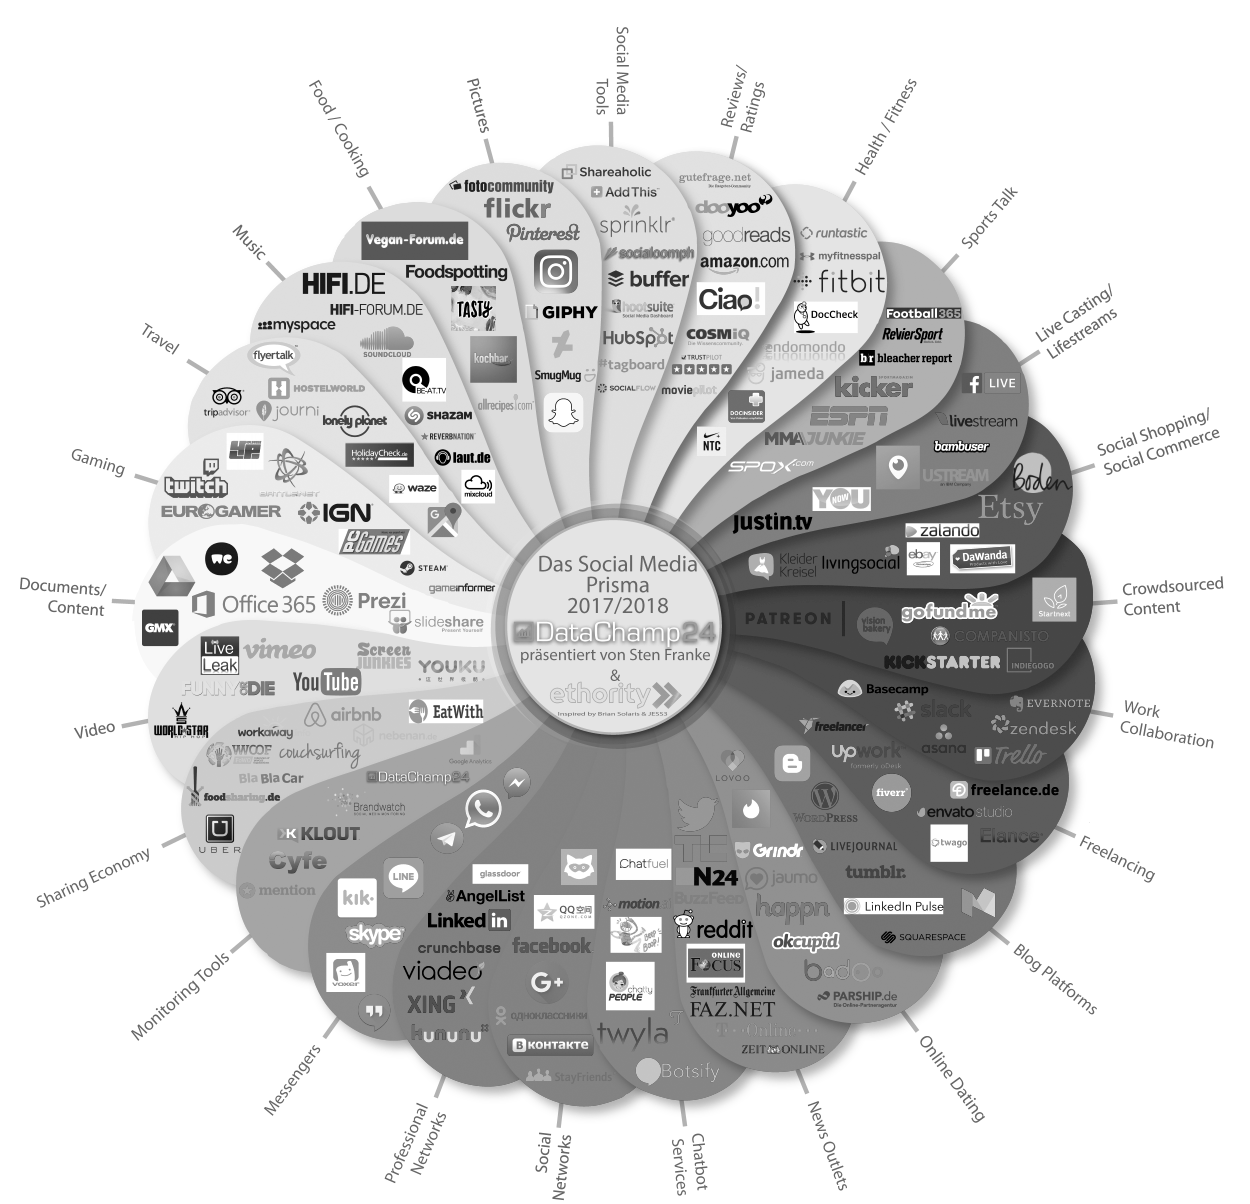
\includegraphics[width=\textwidth]{img/ethority-smp-bw.png}
    \caption{Schaubild zur Übersicht von Social Media Tools aus dem Jahresbericht der Digitalagentur \textit{ethority}. \\ \cite{ethorityprisma2018}}
    \label{fig:socialmediatoolsethority}
\end{figure}

Der Digital-Blog \textit{ethority} stellt regelmäßig ein Schaubild über die meistgenutzten Social Media Plattformen her und veröffentlicht dieses. Der Vollständigkeit halber möchte ich dieses in Abbildung \ref{fig:socialmediatoolsethority} auch zeigen, um die Übersicht zu komplettieren.



Dieses Schaubild verdeutlicht noch einmal die Vielfalt und Masse der Social Media Plattformen, die auf täglicher Basis von bis zu über einer Milliarde Menschen genutzt werden. Wo Privatpersonen, gerade im Hinblick auf die eigene Privatsphäre, sich im Normalfall einer geringeren Anzahl verschiedener Social Media Plattformen bedienen; auch, weil das intendierte Publikum auf vielen Plattformen meist ein limitierter Kreis an Bekannten ist, müssen Unternehmen und Institutionen, die mit Hilfe der Social Media Plattformen ihren Einfluss und ihre Reichweite vergrößern möchten, auf eine Vielzahl von unterschiedlichen Plattformen zurückgreifen.

\section{Die Social Media Kommunikation der Universität Bielefeld}

Die Universität Bielefeld --hier als Beispiel einer Institution-- nutzt ebenfalls diverse Social Media Plattform zur Verbreitung von Inhalten. Auf der Webseite der Universität lassen sich vier der genutzten Plattformen direkt über Icons erreichen.

\begin{figure}[h]
    \centering
    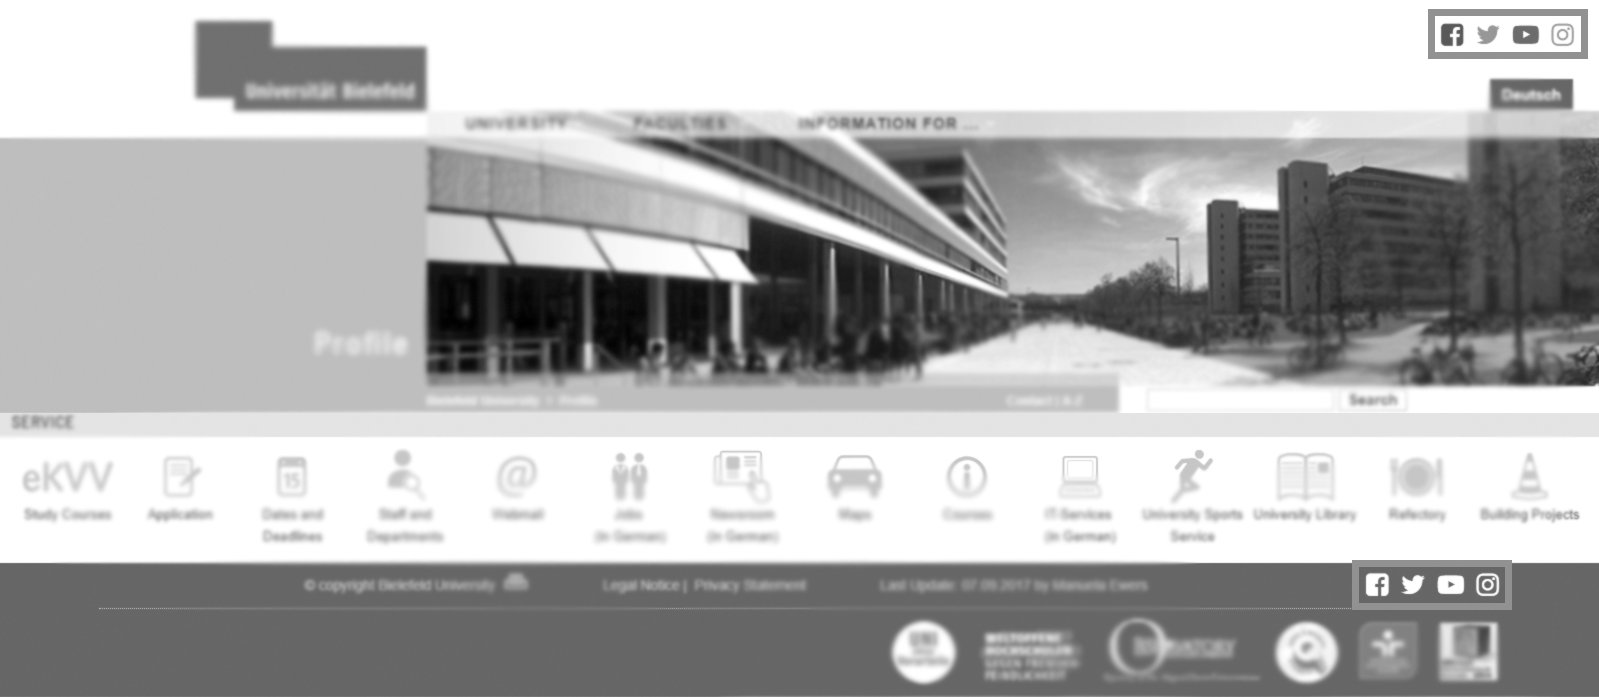
\includegraphics[width=\textwidth]{img/uni-smp-bw.png}
    \caption{Webseite der Universität Bielefeld mit Social Media Menüs im Header und Footer (mit Rechtecken umrandet). Zur besseren Übersicht, wurde der inhaltliche Teil der Webseite entfernt.}
    \label{fig:socialmediatoolsuni}
\end{figure}

Die mehrfache Auflistung der genutzten Plattformen ist im Online Marketing üblich, um bei Webseiten mit längeren Inhalten an möglichst jeder Stelle, auf der sich die Nutzerin/der Nutzer befindet, auf das Angebot verlinken zu können.

In dem sogenannten Social Media Menü werden hier die Angebote Facebook, Twitter, YouTube und Instagram verlinkt. Eine weitere Social Media Plattform, die sich die Universität zu nutze macht, ist ein Blog, der über die Webseite \texttt{\href{http://ekvv.uni-bielefeld.de/blog/uninews/}{ekvv.uni-bielefeld.de/blog/uninews}} erreichbar ist. Eine Besonderheit des Blogs ist, dass sich dieser in verschiedene Unter-Blogs einteilt, über die zum Beispiel auch einzelne Fakultäten, universitäre Einrichtungen oder sogar Einzelpersonen verfügen können. Gegenüber den im Consumer-Bereich häufig genutzten, oben schon angesprochenen, Blogsystemen, wie WordPress oder Blogger, bedienen sich die vom Bielefelder Informationssystem (BIS) verwalteten Blogs dem Blog-System \textit{Apache Blog Roller}.

Ebenfalls für Einrichtungen und Mitarbeiterinnen und Mitarbeiter der Universität zugänglich, ist ein Wiki-System, welches auf der Software \textit{JAMwiki} basiert. Da die Universität als Gesamtinstitution davon jedoch keinen Gebrauch macht, werde ich dieses im weiteren Verlauf außer Acht lassen.

Um aufzeigen zu können, in welchem Maße die verschiedenen Plattformen von den Benutzern genutzt werden, zeige ich die aktuellen Zahlen der Follower aus September 2018 auf. Dabei handelt es sich bei Instagram und Twitter um die Zahlen der Follower, bei YouTube um die Abonnenten des Kanals, und bei Facebook um die Nutzerinnen und Nutzer, die die Facebook-Fanpage der Universität Bielefeld mit einem Like markiert haben.


\begin{figure}[h]    
    \centering
    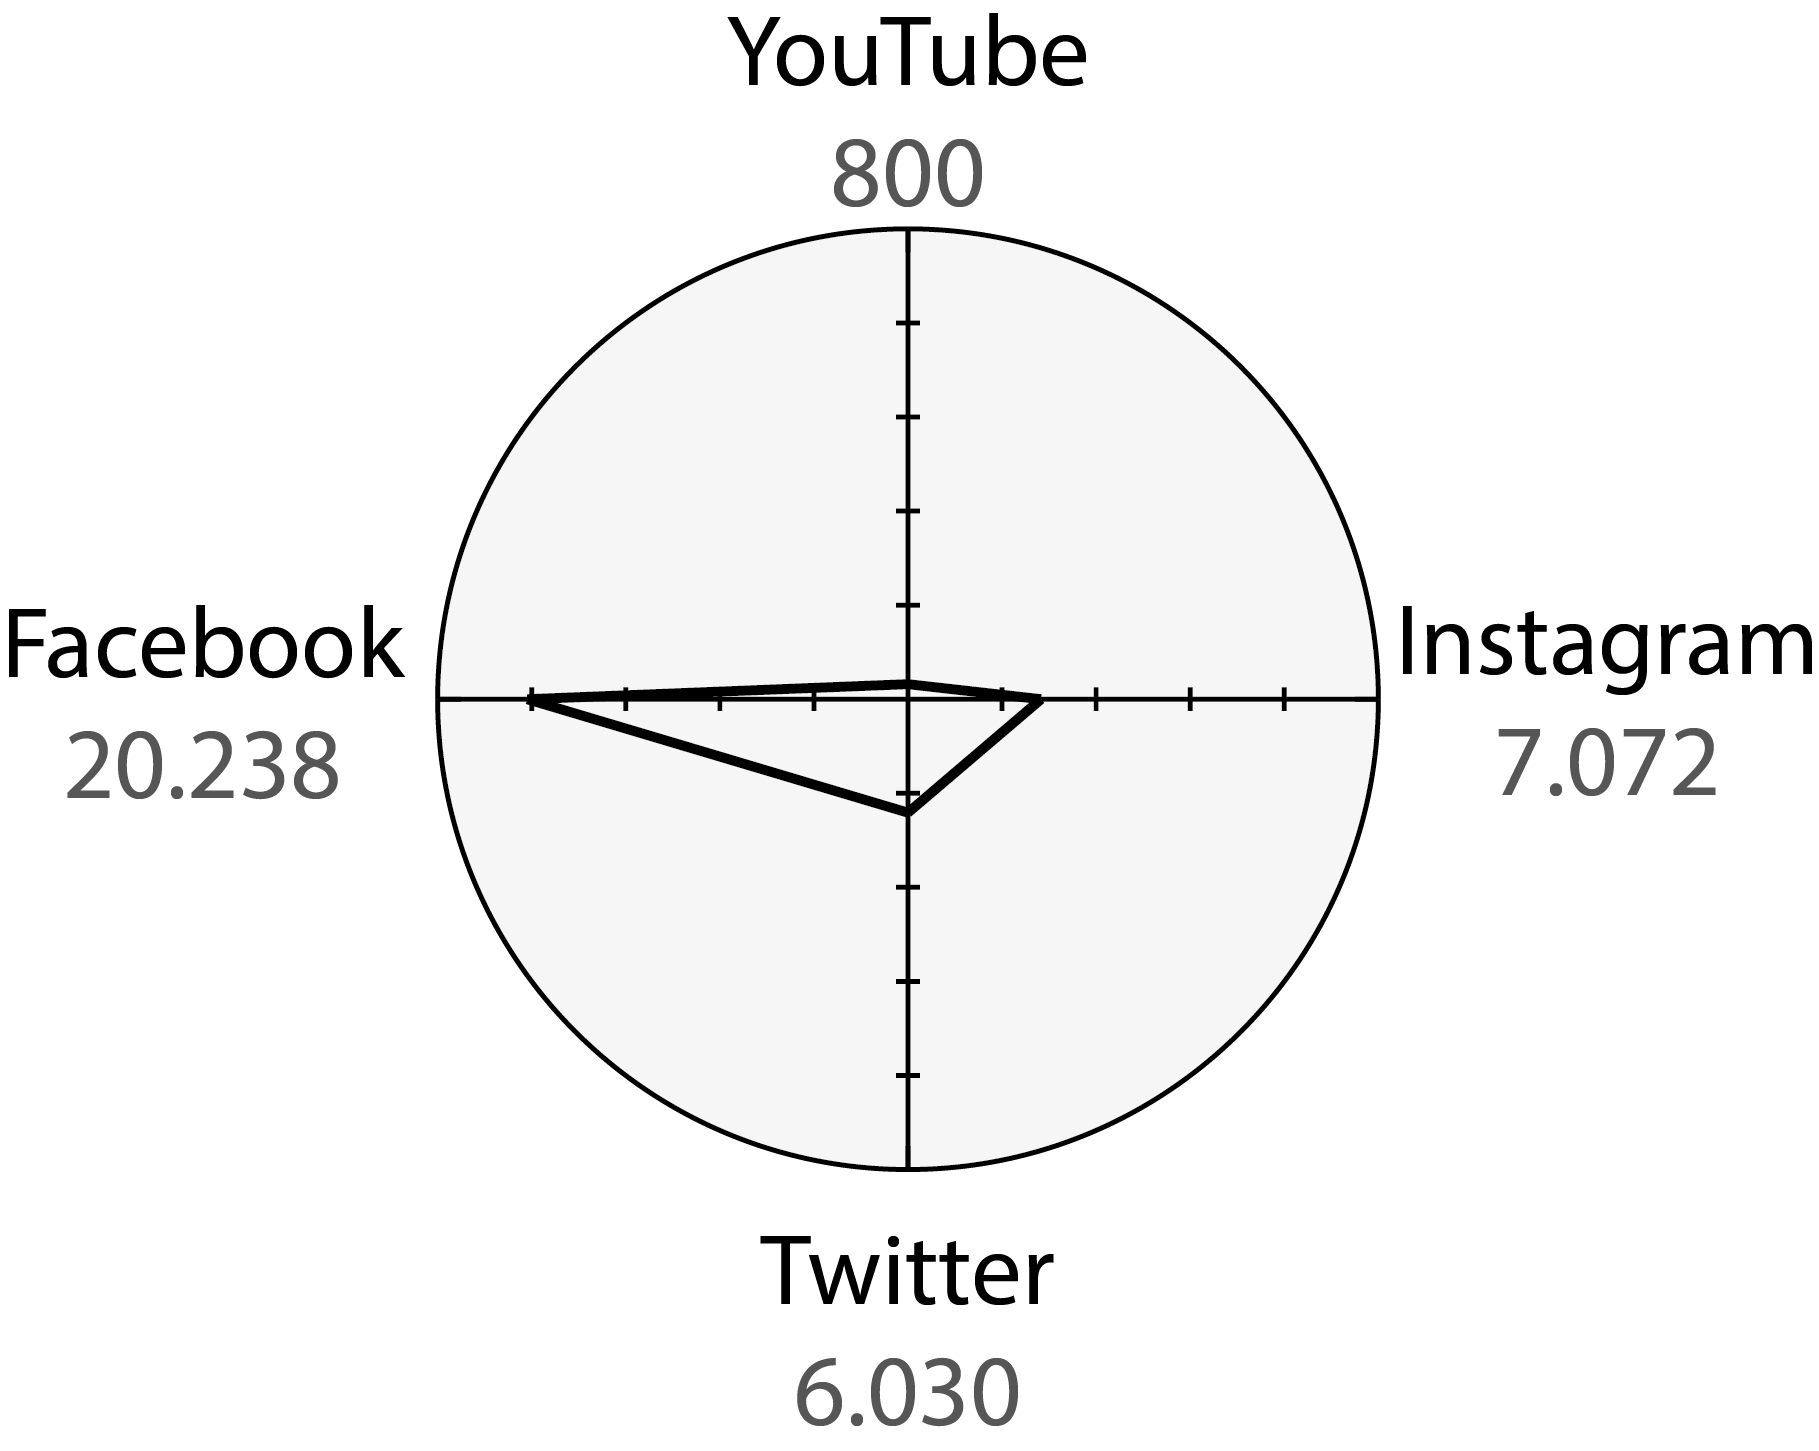
\includegraphics[width=.8\textwidth]{img/posts/follower_gesamt.png}
    \caption{Follower der Social Media Plattformen, die von der Universität Bielefeld genutzt werden in einem Radar-Graphen dargestellt. Ein deutlicher Überhang der Plattformen Facebook, Twitter und Instagram gegenüber dem YouTube-Kanal ist zu erkennen (Stand: September 2018).}
    \label{fig:follower}
\end{figure}

\begin{table}[h]
    \centering
        \caption{Prozentuale Verteilung der Follower der von der Universität Bielefeld genutzten Social Media Plattformen.}
        \begin{tabular}{*{5}{l}}
        Facebook & Universitäts-Blog & Instagram & YouTube & Twitter \\
        \hline
        59,28 \% & nicht messbar & 20,71 \% & 2,34 \% & 17,66 \%
        \end{tabular}
    \label{tab:followerprozent}
\end{table}

Insgesamt 34.140 Follower hat die Universität Bielefeld auf ihren Social Media Plattformen. Davon nutzen mit knapp 60 \% Facebook die meisten, und mit nur knapp 2,3 \% YouTube die wenigsten Follower. Twitter nimmt knapp 18 \%, und Instagram knapp 21 \% der Gesamtfollower ein. Dabei ist, wie oben angegeben, zu beachten, dass die Zahl der Blog-Follower nicht messbar ist, da dieser unter anderem auch per RSS-Feed zugänglich ist, welcher die Besucherzahlen nicht preisgibt.

\section{Forschung -- Jan-Hinrik Schmidt}
\label{sec:aktuelleforschung}

Das folgende Kapitel dient der Übersicht des aktuellen Standes der Social Media Forschung. Ausgehend von Jan-Hinrik Schmidts \textit{"Was ist neu am Social Web?"}, werde ich in diesem Kapitel im Allgemeinen auf Schmidts Forschung im Bereich der sozialen Medien eingehen und seine Begriffswahl erläutern. Danach widme ich mich im Speziellen dem von ihm geprägten Kommunikations-Modell, das die Begrifflichkeit dreier Leistungen definiert, die durch Anwendungen im Social Web unterstützt werden \cite{schmidt2008neu}.

\subsection{Social Media wird zu \textit{Social Web}}

Die Social Media Kommunikation lässt sich dem Namen entsprechend relativ einfach innerhalb der Linguistik in den Bereich der Kommunikationswissenschaft einordnen. Als Kommunikationswissenschaftler mit Wurzeln in der Soziologie kritisiert Jan-Hinrik Schmidt den von O'Reilly (2004) geprägten Begriff des Web 2.0 und postuliert, jene Bezeichnung mit dem Begriff Social Web zu ersetzen. Die Bezeichnung 2.0, die sich der Notation der üblichen Versions-Nummerierung in Computer-Anwendungen bedient, vermittle grundlegende und schrittartige Veränderungen. Die zu beobachtenden Veränderungen verlaufen jedoch fließend, weshalb Schmidt die Versions-Nummerierung für ungünstig hält und einen Gegenvorschlag liefert.

Der Begriff \textit{Social Web} soll die Wichtigkeit der sozialen Aspekte in den Vordergrund stellen, da in der Zeit des Produsers\footnote{Ein Produser nimmt in einem einzigen Netzwerk sowohl die übliche Rolle des Rezipienten als auch die eher unüblichere Rolle des Produzenten gleichzeitig ein.} die Internet-Kommunikation weit über die Kommunikation von Mensch zu Maschine hinausgeht und immer mehr Nutzerinnen und Nutzer zu solchen Produsern werden, statt die sozialen Medien einzig zur Rezeption zu nutzen. Das Weglassen der Versions-Nummerierung soll den stetigen Wandel der sozialen Medien verdeutlichen. Im weiteren Verlauf dieser Arbeit möchte ich mich an dieser Begrifflichkeit orientieren.

"Wie jede andere Form des sozialen Handelns auch ist die Nutzung des Social Web durch die Dualität von Struktur und Handeln gekennzeichnet", so Schmidt. Diese Dualität, die Schmidt mit \cite{giddens1988konstitution} zitiert kann ebenfalls auf die Analyse von Social Web Kommunikation angewandt werden (vgl. \cite{schmidt2006social} \& \cite{schmidt2006weblogs}). Dabei ist, um das Handeln und die sozialen Strukturen zu verbinden, das Konzept der Nutzungspraxis von entscheidender Bedeutung.

Schmidt nennt dieses Konzept die Manifestation gerahmter Nutzungsabsichten, und erläutert die erwähnte Rahmung im Detail. Zu ihr gehören unterschiedlich explizite und sanktionierbare Verwendungsregeln; von selbst erstellten Verhaltenskodizes -- in zum Beispiel privaten Chat-Gruppen -- über Geschäfts- und Nutzungsbedingungen von Social Web Plattformen, bis hin zu juristischen Regelungen, wie sie beispielsweise über das Inkrafttreten der EU Datenschutzgrundverordnung (EU DSGVO) \cite{eurlex2016} im Mai diesen Jahres großes Aufsehen erregt haben. Neben diesen Verwendungsregeln spielen zwei weitere strukturelle Dimensionen eine Rolle: Zum einen der Code, der die softwaretechnischen Grundlagen einer Social Web Anwendung festlegt, indem er die Möglichkeiten, die eine Anwendung der Nutzerin/dem Nutzer bietet, überhaupt erst erschafft; jedoch gleichzeitig auch einschränkt. (Für letztere Funktionsweise des Codes ist die Zeichen-Limitierung von Beiträgen auf Twitter ein hervorragendes Beispiel.) Zum anderen die Relationen, die im hypertextuellen Zusammenhang die Verknüpfungen von Stellen innerhalb eines Dokuments -- sogenannte \textit{intra}textuelle Hyperlinks -- oder aber auch die Verknüpfungen von verschiedenen Dokumenten miteinander -- sogenannte \textit{inter}textuelle Hyperlinks -- darstellen.

Von der Beschreibung der Nutzungspraxis kommt Schmidt zu den Leistungen, die das Social Web unterstützt. Diese Leistungen stellen den Kern der Forschung dar, auf die diese Arbeit aufbaut, und auf die ich im folgenden Kapitel eingehen werde.

\subsection{Modell der Social Web Kommunikation}
\label{sec:jhsforschung}

Drei Funktionen werden nach Schmidt von den Anwendungen im Social Web unterstützt. Hierbei handelt es sich um Formen des Managements der persönlichen Öffentlichkeit einer Nutzerin/eines Nutzers. 

Die erste Funktion ist das \textit{Identitätsmanagement}. Innerhalb des Identitätsmanagements macht die Nutzerin/der Nutzer spezifische Teile der eigenen Person publik, was zur Entwicklung der eigenen persönlichen Öffentlichkeit beiträgt. Die von Schmidt angesprochene Leistung, die das Identitätsmanagement erbringen kann, ist das selektive Präsentieren der eigenen Person. Die Nutzerin/Der Nutzer kann Aspekte der eigenen Person vor der Veröffentlichung filtern, und bleibt somit gewissermaßen in Kontrolle. Unter prototypische Anwendungen, die das Identitätsmanagement unterstützt, fallen beispielsweise Blogs, Pod- und Videocasts, Nutzerprofile auf Social Web Plattformen und Video-Plattformen, wie YouTube und Vimeo. Über diese Anwendungen können bestimmte Aspekte der eigenen Person, wie Meinungen, Interessen, Weltanschauungen, Wissen, etc. präsentiert werden.

Die zweite Funktion ist das \textit{Beziehungsmanagement}. Hierbei werden die Anwendungen des Social Web dazu genutzt noch nicht existente Beziehungen zu knüpfen und vorhandene Beziehungen auszubauen oder zu verändern. Das Netzwerken, sowohl privat über Plattformen wie Facebook als auch auf professioneller, beruflicher Ebene, beispielsweise über LinkedIn und XING, ist in Schmidts Modell die soziale Form der Hyperlinks. Diese stellen, wie oben bereits angesprochen, intra- oder intertextuelle Verknüpfungen her. Übertragen auf die persönliche Öffentlichkeit, stellen diese also interpersonelle Beziehungen her, indem man zum Beispiel über Facebook eine andere Nutzerin/einen anderen Nutzer als Freundin/Freund hinzufügt.

Die dritte Funktion der Social Web Anwendungen ist das \textit{Informationsmanagement}. Bei diesem geht es sowohl um die Produktion als auch die Rezeption von Informationen. Prototypische Anwendungen sind zum Beispiel Wikis. Aber auch kollaborative Wissensplattformen, wie diverse Reddit Unterforen, oder die von Y Combinator erstellte Plattform \textit{Hacker News}, die für Programmierer  -- und auch für die Open Source Bewegung -- Technik-Nachrichten aggregiert, zählen zu den prototypischen Anwendungen, die die Funktion des Informationsmanagements unterstützen. Die vom Informationsmanagement erbrachten Leistungen umfassen neben dem Auffinden und der Rezeption von Informationen auch deren Verwaltung. Letztere Leistung ist besonders in der Open Source Bewegung und in der Gruppe der SystemadministratorInnen häufig durch sogenannte \textit{Personal Knowledge Bases} -- also private Wissenssammlungen -- abgedeckt. Eine solche Knowledge Base kann ebenfalls ein privat angelegtes Wiki sein, dass dann einzig zur Verwaltung eigenen Wissens dient.

%\newpage
\section{Forschungsfragen und Hypothesen}
\label{sec:hypothesen}

In diesem Abschnitt werde ich aus den vorangegangenen Kapiteln Forschungsfragen herleiten und diese zu Hypothesen formen. Dabei gehe ich sowohl auf die Nutzerinnen- und Nutzerseite der Social Web Plattformen als auch auf die in \ref{sec:aktuelleforschung} erarbeiteten Forschungsgrundlagen ein, um die Hypothesen zu begründen.

Wie in \ref{sec:jhsforschung} deutlich wurde, ist das Modell nach Jan-Hinrik Schmidt ein auf die Einzelperson zugeschnittenes Modell. Wo einige Aspekte des Social Web, wie zum Beispiel der der Social Web Anwendungen zugrunde liegende Code (vgl. \cite{schmidt2008neu}), für jede Art von Nutzung -- also auch die, der Institution -- gelten, spielt der Kern des Modells auf die Einzelnutzung, zum Beispiel durch das Zugänglich-Machen der eigenen Person durch Artikulation der persönlichen Meinung, oder auch die Angabe von Freundschaften auf Facebook ab \cite{schmidt2008neu}. Diese Beispiele des Identitätsmanagements und des Beziehungsmanagements lassen sich typischerweise mit der Einzelnutzung der Social Web Plattformen in Verbindung bringen. Der Institution Universität sind diese beiden Formen des Selbstmanagements weniger eindeutig zuzuordnen, da die Institution als solche auf andere Arten von Beziehungen angewiesen ist, als eine Einzelperson. 

Ist das Modell nach Jan-Hinrik Schmidt dennoch auf die Social Web Kommunikation der Universität Bielefeld anwendbar? Und ist es möglich, die Social Web Beiträge, die die Universität Bielefeld veröffentlicht, eindeutig den in Abschnitt \ref{sec:jhsforschung} eingeführten Leistungen zuzuordnen? In Kapitel \ref{chap:Empirie} möchte ich diesen Fragen nachgehen. \smallskip

Aus den stark auf die Einzelperson zugeschnittenen Eigenschaften des Kommunikationsmodells nach Jan-Hinrik Schmidt, und den grundlegend verschiedenen Beschaffenheiten von persönlichen und institutionellen Öffentlichkeiten, geht die Hypothese dieser Arbeit hervor, dass die Anwendbarkeit des Modells auf die Social Web Kommunikation der Universität Bielefeld nicht vollständig gegeben ist, und das Modell einer Überarbeitung oder Erweiterung bedarf, um auch institutionelle Social Web Kommunikation abdecken zu können.


\chapter{Empirische Verarbeitung}
\label{chap:Empirie}

\section{Methodik}
\label{sec:Methodik}

Im folgenden Kapitel werde ich die der Studie zugrunde gelegten Daten präsentieren, ihre Auswahl begründen, und ihre Beschaffung und Bereinigung beschreiben. Im Anschluss werde ich die Social Web Beiträge nach den in \ref{sec:jhsforschung} erarbeiteten Kriterien in die Funktionsgruppen des Modells von Jan-Hinrik Schmidt einordnen, so dies denn möglich ist.

\subsection{Daten}
\label{sec:Daten}

\subsubsection{Datenauswahl}
\label{sec:Datenauswahl}

Der untersuchte Datensatz umfasst die Social Web Beiträge, die von der Universität Bielefeld selbst im Zeitraum vom 01. Juli 2018 bis einschließlich 31. Juli 2018 jeweils auf den Plattformen Instagram, YouTube, Twitter, Facebook, Universitäts-Blog veröffentlicht worden sind. Der einmonatige Zeitraum wurde gewählt, um eine noch analysierbare, jedoch aussagekräftige Beitrags-Menge zu erhalten. Der spezifische Zeitraum liegt im Übergang von Vorlesungszeit zu vorlesungsfreier Zeit, damit ein eventueller Unterschied zwischen den beiden Perioden dargestellt werden kann.

\subsubsection{Beschaffung}
\label{sec:Datenbeschaffung}

Die Facebook-Beiträge wurden mit Hilfe der Facebook Graph API\footnote{Facebook Graph API - \url{https://developers.facebook.com/tools/explorer} - Eine Programmierschnittstelle zur automatisierten Datenbeschaffung} im in der automatisierten Datenverarbeitung üblichen JSON-Format heruntergeladen, um die Text-Beiträge von der grafischen Oberfläche unabhängig darstellen zu können. Für die Twitter-Beiträge wurde die Twitter Search API\footnote{Twitter Search API - \url{https://twitter.com/search-advanced}} genutzt, um ebenselben Effekt zu erzielen. Aufgrund der weniger umfangreichen Beitragszahl, wurde die Liste der YouTube-Beiträge händisch erstellt. Selbes gilt für die Instagram-Beiträge. Die Blog-Beiträge des Universitäts-Blogs wurden ebenfalls händisch heruntergeladen, da das genutzte Blogsystem keine Programmierschnittstelle zur Verfügung stellt.

Zusätzlich zu den Text-Varianten, wurden grafische Darstellungen aller Beiträge erstellt und im Anhang archiviert.

\subsubsection{Bereinigung}
\label{sec:Datenbereinigung}

Die Facebook-Beiträge wurden so bereinigt, dass nur noch Inhalt, Reaktionszahlen (Like, etc.), Kommentarzahlen und eine Info vorhanden sind, ob dem Text-Beitrag ein weiteres Medium hinzugefügt wurde; und wenn ja, welches (Bild, Video, Link, Veranstaltungseinladung). Bei den Twitter-Beiträgen wurden neben dem Inhalt die Interaktionsdaten zu Kommentaren, Retweets und Likes aufgenommen. Für die Instagram-Beiträge wurden die Beschreibung des Bildes/Videos, die Zahlen der Likes und die Zahlen der Kommentare aufgenommen. Die YouTube-Videos wurden mit Videobeschreibung, View- und Like-, sowie Kommentarzahlen notiert. Da beim Universitäts-Blog die Kommentarfunktion nicht aktiviert ist, wurden hier nur die Beiträge in den Datensatz aufgenommen.

\subsubsection{Datensatz}
\label{sec:Datensatz}

Der gesamte Datensatz umfasst 105 Beiträge, von denen in aufsteigender Reihenfolge sieben auf Twitter, elf auf YouTube, 22 auf Instagram, 29 im Universitäts-Blog und 36 auf Facebook veröffentlicht wurden.

\begin{figure}[h]
    \centering
    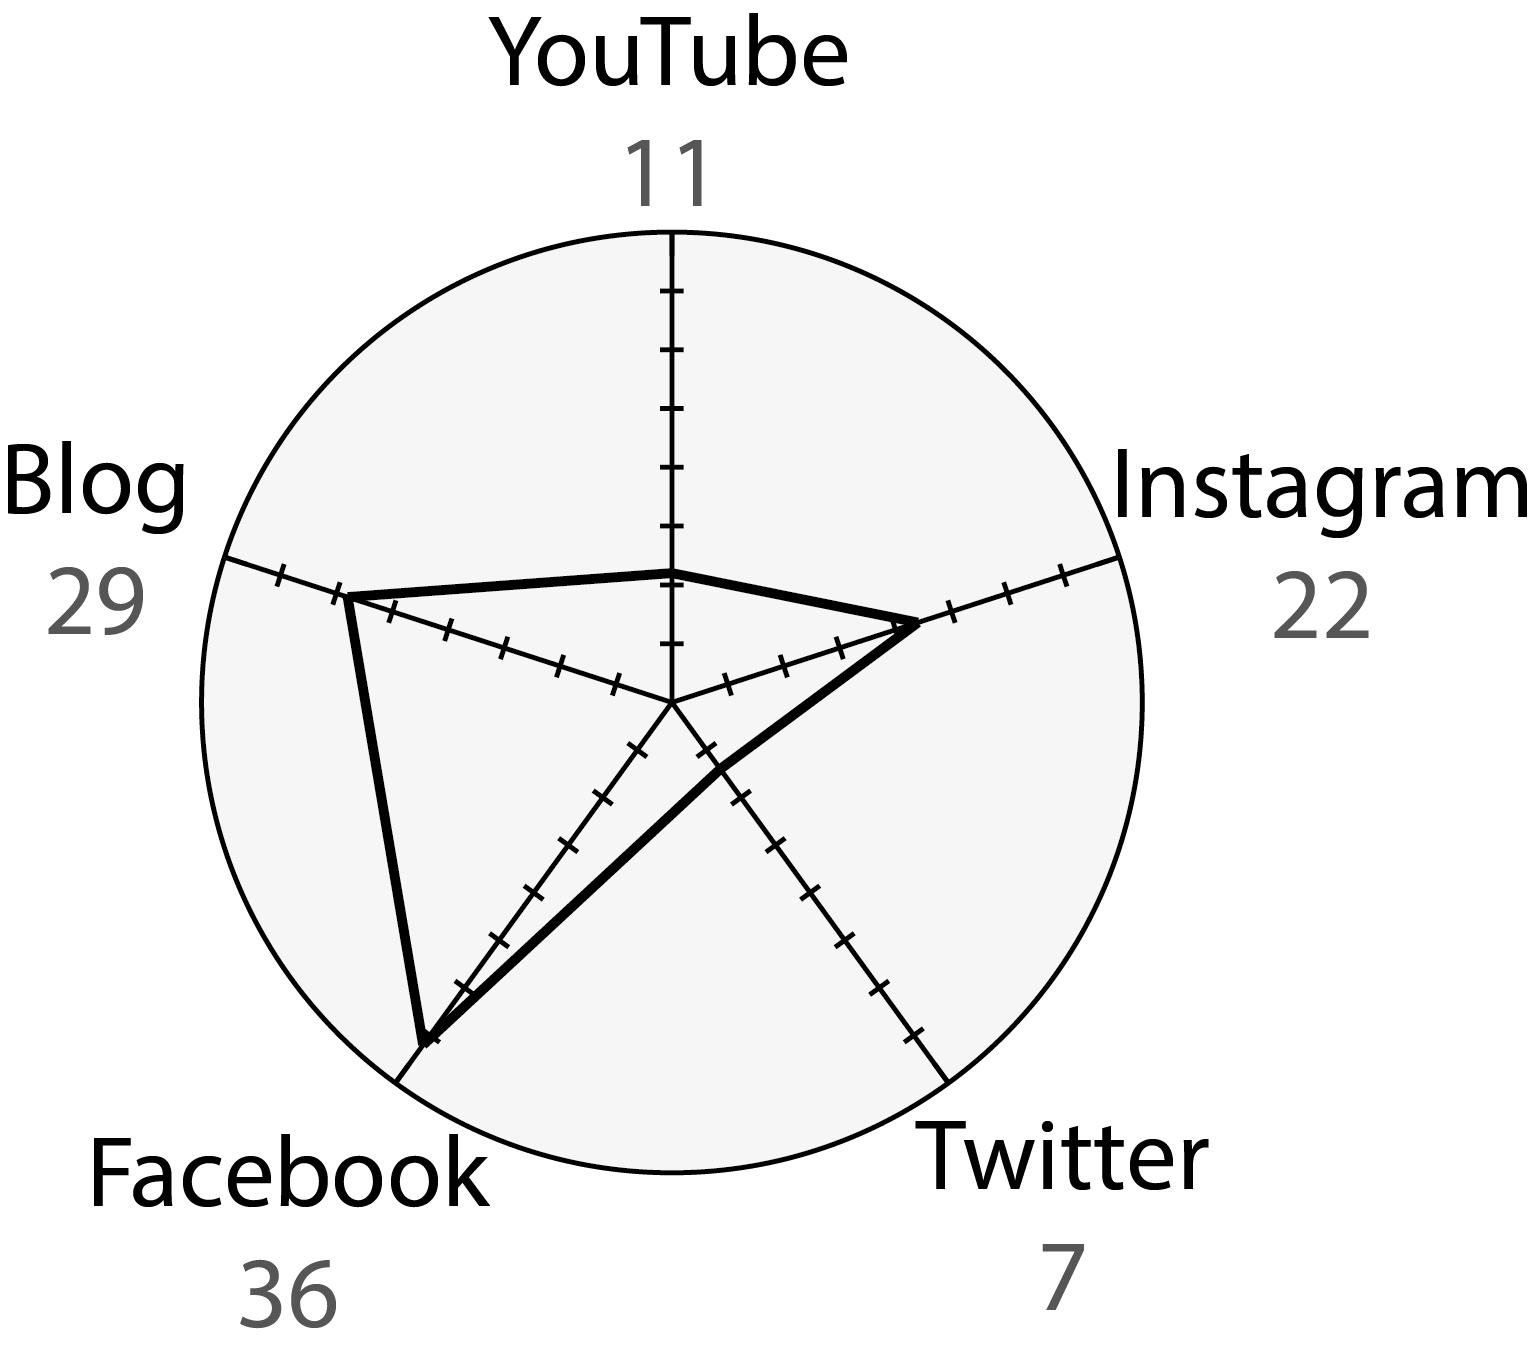
\includegraphics[width=.6\textwidth]{img/posts/posts_gesamt.png}
    \caption{Social Web Beiträge der Universität Bielefeld im Juli 2018. Der Radar-Graph zeigt einen Überhang an Facebook- und Blog-Beiträgen und ein Minimum an Twitter-Beiträgen.}
    \label{fig:socialmediaposts}
\end{figure}  

Dabei sind die Blog-Beiträge, mit durchschnittlich knapp 400 Worten, die längsten Beiträge, wie dem Boxplot in Abbildung \ref{fig:wortlaengebl} zu entnehmen ist.

\begin{figure}[h]
    \centering
    \includegraphics[width=\textwidth]{img/plots/bl.png}
    \caption{Textlänge der Blog-Beiträge in einem Boxplot-Diagramm. Die gestrichelte Linie zeigt den Durchschnitt, die darüber liegende Linie den Median an. Das Minimum liegt bei 49, das Maximum bei 688 Worten.}
    \label{fig:wortlaengebl}
\end{figure}

Die Beitragslängen im Blog reichen von 49 bis zu 688 Worten, erreichen bei etwa 390 Worten den Durchschnitt und bei knapp 404 Worten den Median. Daraus ergibt sich eine Standardabweichung von 182.28.

\begin{figure}[h]
    \centering
    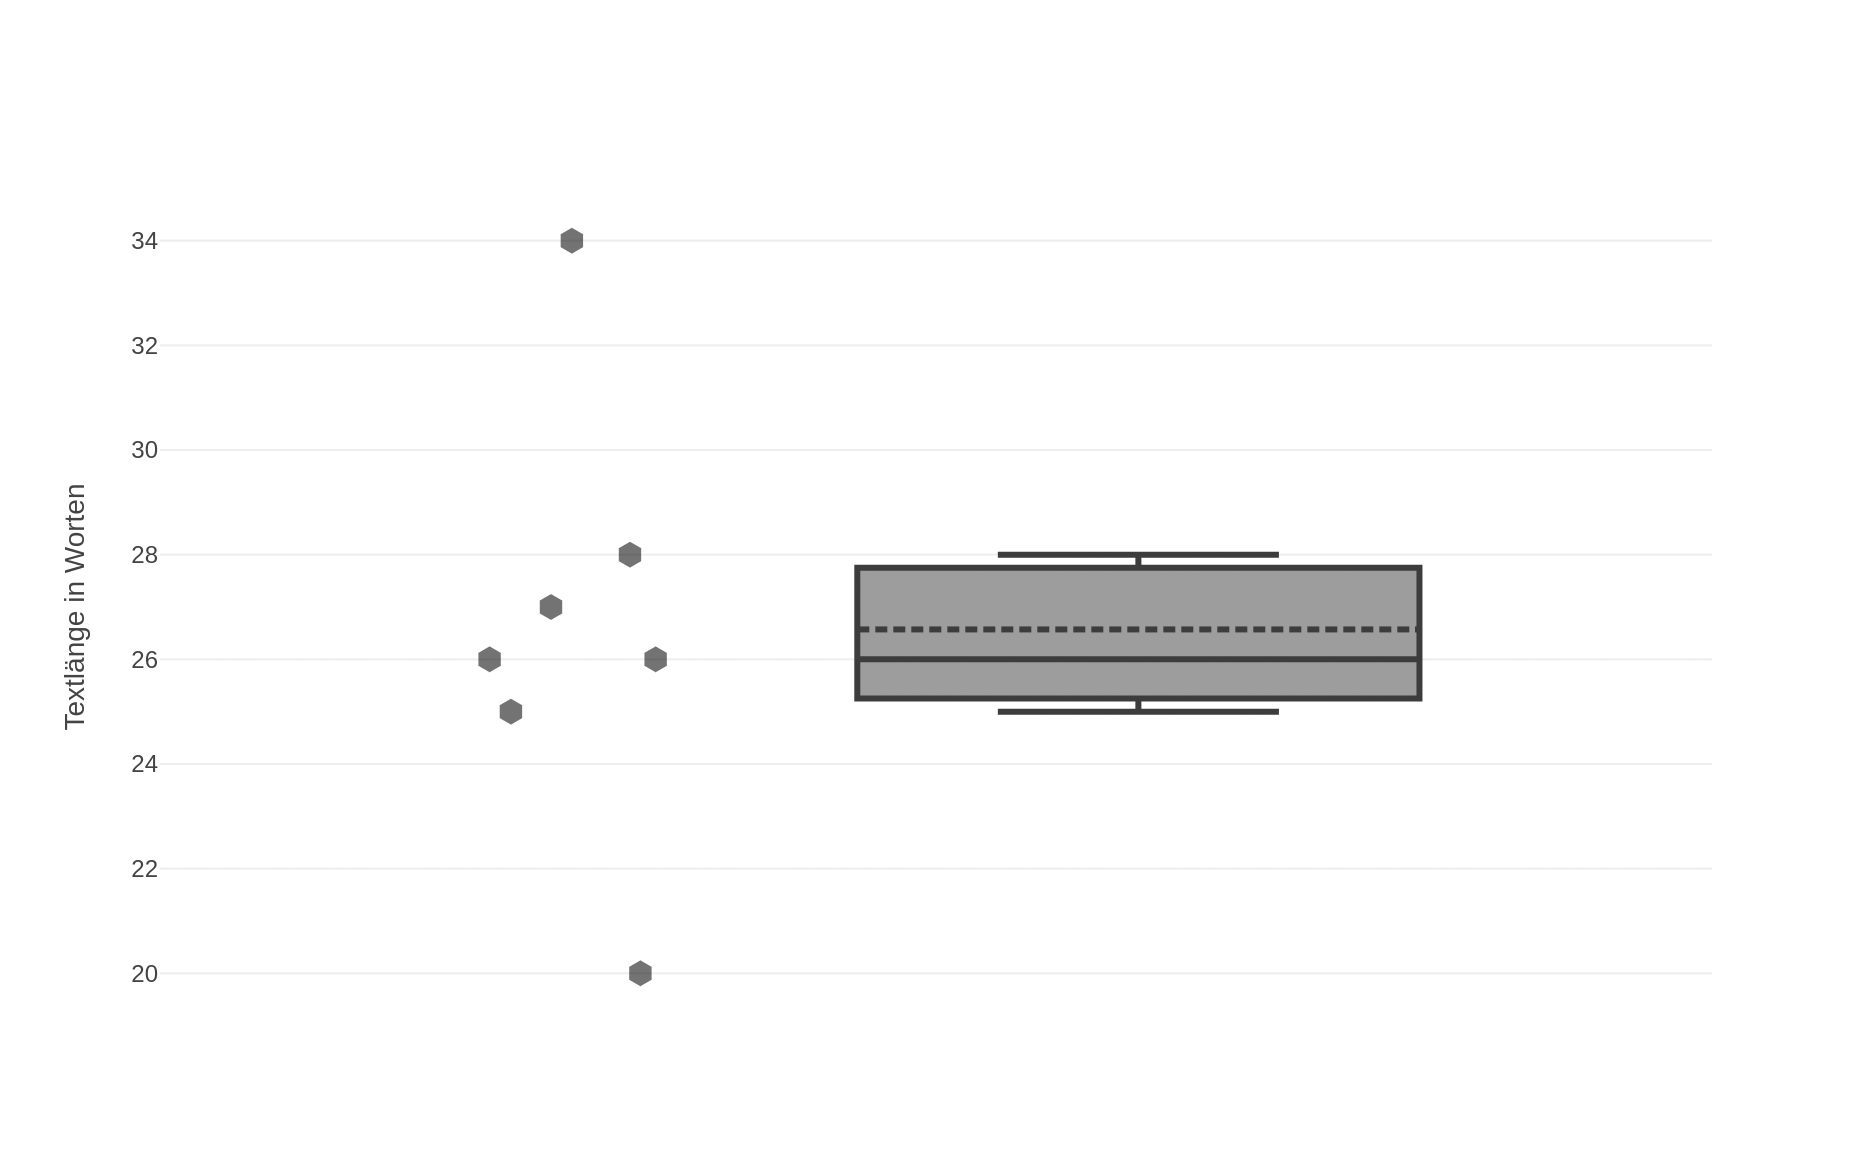
\includegraphics[width=\textwidth]{img/plots/tw.png}
    \caption{Textlänge der Twitter-Beiträge in einem Boxplot-Diagramm, welche den technischen Einschränkungen der Plattform nach erwartungsgemäß eine niedrige Standardabweichung aufzeigen.}
    \label{fig:wortlaengetw}
\end{figure}

\begin{figure}[h]
    \centering
    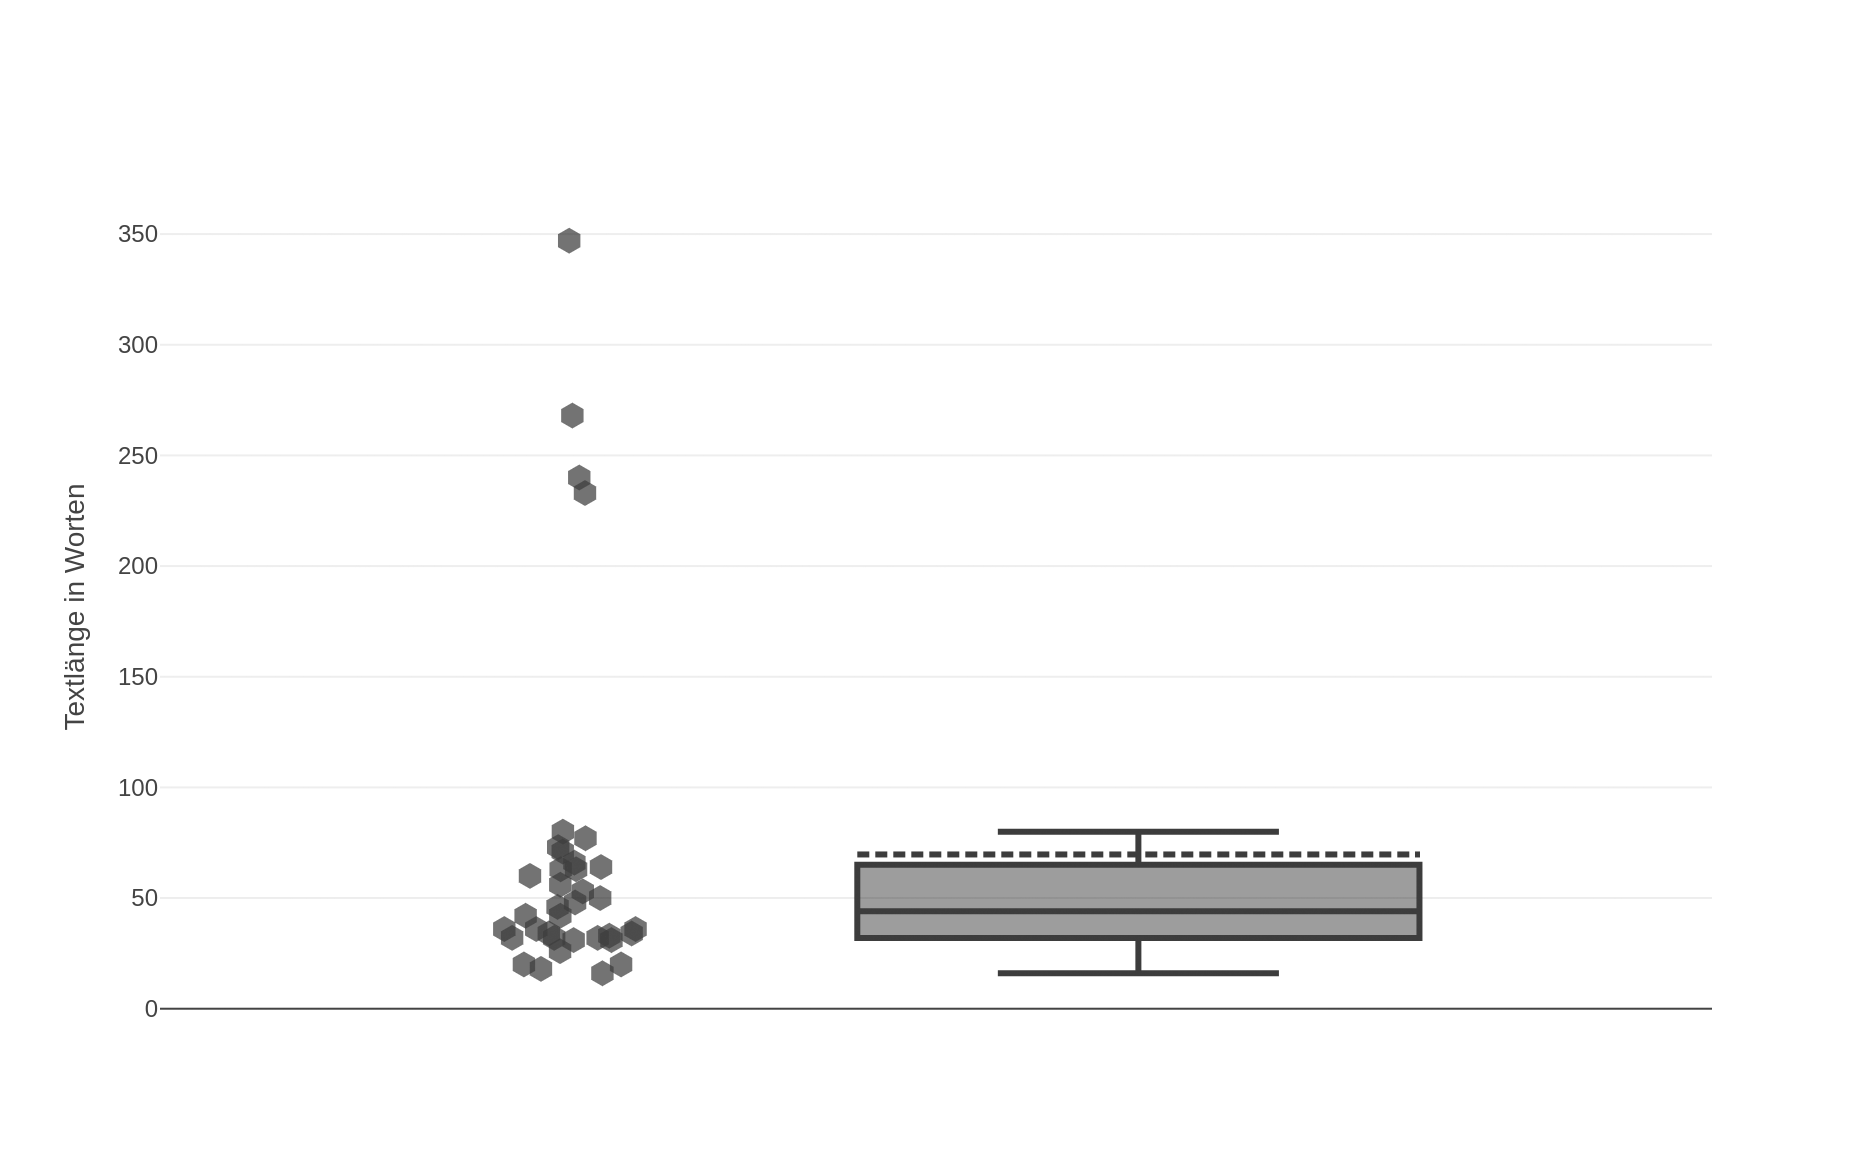
\includegraphics[width=\textwidth]{img/plots/fb.png}
    \caption{Textlänge der Facebook-Beiträge. In der Box ist der Median durch die durchgezogene Linie angezeigt. Die gestrichelte Linie zeigt den Durchschnitt, der durch die Ausreißer am oberen Rand des Spektrums über die Box hinausgeht. Hier reicht die Textlänge von 16 Worten bis hin zu 347 Worten}
    \label{fig:wortlaengefb}
\end{figure}

In den Abbildungen \ref{fig:wortlaengetw} \& \ref{fig:wortlaengefb} sind Boxplots der Textlängen von respektive Twitter- und Facebook-Beiträgen dargestellt.

Die Twitter-Beiträge bewegen sich zwischen 20 und 34 Worten. Der Durchschnitt liegt bei knapp 27 und der Median bei knapp 26 Worten. Die Standardabweichung ist mit knapp vier Worten sehr viel kleiner als die der Blog- und Facebook-Beiträge. Dies ist sehr deutlich in Abbildung \ref{fig:wortlaengetw} zu erkennen.

Wie in Abbildung \ref{fig:wortlaengefb} zu sehen, reichen die Beiträge von Facebook von 16 bis zu 347 Worten. Im Durchschnitt hat ein Facebook-Beitrag knapp 70 Worte. Der Median liegt bei 44 und die Standardabweichung mit 76 Worten zwischen denen der Twitter- und Blog-Beiträge. Alle Ausreißer der Facebook-Beiträge sind dem Beitrags-Format \textit{Meine Uni - Mein Thema} zuzuordnen.

Da es sich bei YouTube und Instagram im Kern nicht um textbasierte Plattformen handelt, wurden die oben aufgezeigten Statistiken für diese Plattformen nicht ausgeführt.


\subsection{Einteilung der Social Web Posts der Universität Bielefeld in die Management-Leistungen nach Jan-Hinrik Schmidt}
\label{sec:jhseinteilung}

Die auf Text basierten Social Web Beiträge der Universität Bielefeld sollen in diesem Abschnitt in die von Jan-Hinrik Schmidt eingeführten Leistungen Identitätsmanagement (\texttt{ID}), Beziehungsmanagement (\texttt{BEZ}) und Informationsmanagement (\texttt{INFO}) eingeteilt werden. In den erstellten Tabellen sind den Beiträgen jeweils UIDs (Unique Identifiers) zugeordnet worden. Diese setzen sich nach dem Schema \texttt{SWP\_D\_C} zusammen. \texttt{SWP} ist das Kürzel der Social Web Plattform; \texttt{FB} für Facebook, \texttt{BL} für den Universitäts-Blog und \texttt{TW} für Twitter. \texttt{D} ist die zweistellige Darstellung des Tages innerhalb des Monats Juli 2018. \texttt{C} ist ein sogenannter Counter, also eine Zählvariable; für den Fall, dass an einem Tag mehrere Beiträge auf ein und derselben Plattform veröffentlicht wurden.

\texttt{TW\_16\_03} wäre demnach der dritte Beitrag, der am 16. Juli 2018 auf der Twitter-Seite der Universität Bielefeld veröffentlicht wurde.

In den Spalten \texttt{ID}, \texttt{BEZ} und \texttt{INFO} wird jeweils ein \texttt{X} eingetragen, wenn der Beitrag der jeweiligen Management-Leistung zugeordnet werden kann. Ist dies nicht der Fall, wird die Tabellen-Zelle leer gelassen.

\subsubsection{Facebook}

In der folgenden Tabelle \ref{tab:kategoriefb} sind in den Spalten die UIDs der Facebook-Beiträge der Universität Bielefeld aus dem Juli 2018 eingetragen, die sich wie oben in \ref{sec:jhseinteilung} beschrieben zusammensetzen. In den drei Datenzeilen ist eingetragen, ob der entsprechende Beitrag der angegebenen Management-Leistung zugeordnet werden kann. Wie folgend auch in \ref{fig:kategoriefb} zu sehen, ließen sich 20.9 \% der Beiträge zum Identitätsmanagement, 18.6 \% dem Beziehungsmanagement, und 60.5 \% dem Informationsmanagement zuteilen. Zu beachten ist, dass sowohl Einfach- als auch Mehrfachkategorisierungen möglich waren. Wie im rechten Teil der Abbildung \ref{fig:kategoriefb} zu sehen, konnten 16.7 \% aller Beiträge keiner der drei Management-Leistungen zugeordnet werden. 47.2 \% der Beiträge waren eindeutig zuordenbar; 36.1 \% konnten mehreren Kategorien zugeordnet werden.

\begin{table}[H]
    \caption{Facebook Beiträge der Universität Bielefeld im Juli 2018 und ihre Zuordnung zu den Management-Leistungen nach Schmidt.}
\resizebox{\textwidth}{!}{%
\begin{tabular}{*{36}{c|}c}
& \rotatebox{270}{FB\_02\_01} & \rotatebox{270}{FB\_02\_02} & \rotatebox{270}{FB\_03\_01 } & \rotatebox{270}{FB\_04\_01} & \rotatebox{270}{FB\_04\_02} & \rotatebox{270}{FB\_05\_01} & \rotatebox{270}{FB\_05\_02} & \rotatebox{270}{FB\_05\_03} & \rotatebox{270}{FB\_06\_01} & \rotatebox{270}{FB\_06\_02} & \rotatebox{270}{FB\_09\_01} & \rotatebox{270}{FB\_10\_01} & \rotatebox{270}{FB\_11\_01} & \rotatebox{270}{FB\_12\_01} & \rotatebox{270}{FB\_12\_02} & \rotatebox{270}{FB\_13\_01} & \rotatebox{270}{FB\_13\_02} & \rotatebox{270}{FB\_16\_01} & \rotatebox{270}{FB\_17\_01} & \rotatebox{270}{FB\_18\_01} & \rotatebox{270}{FB\_18\_02} & \rotatebox{270}{FB\_19\_01} & \rotatebox{270}{FB\_20\_01} & \rotatebox{270}{FB\_20\_02} & \rotatebox{270}{FB\_23\_01} & \rotatebox{270}{FB\_24\_01} & \rotatebox{270}{FB\_24\_02} & \rotatebox{270}{FB\_25\_01} & \rotatebox{270}{FB\_26\_01} & \rotatebox{270}{FB\_26\_02} & \rotatebox{270}{FB\_27\_01} & \rotatebox{270}{FB\_27\_02} & \rotatebox{270}{FB\_27\_03} & \rotatebox{270}{FB\_30\_01} & \rotatebox{270}{FB\_30\_02} & \rotatebox{270}{FB\_31\_01} \\
\hline
 ID & &  &  &  &  & X & X &  &  & X &  & X & X &  &  &  & X &  &  &  &  &  &  &  &  &  &  &  & X &  &  & X &  &  & X &  \\
 \hline
 BEZ & & X & X & X &  & X &  & X & X &  &  & X &  &  &  &  &  &  &  &  &  &  & X &  &  &  &  &  &  &  &  &  &  &  &  &  \\
 \hline
 INFO & & X & X & X & X &  & X & X & X & X &  & X &  & X & X & X & X &  & X &  &  & X &  & X &  & X & X & X & X & X & X & X & X &  & X & X
\end{tabular}%
}
\label{tab:kategoriefb}
\end{table}

\begin{figure}[H]
    \centering
    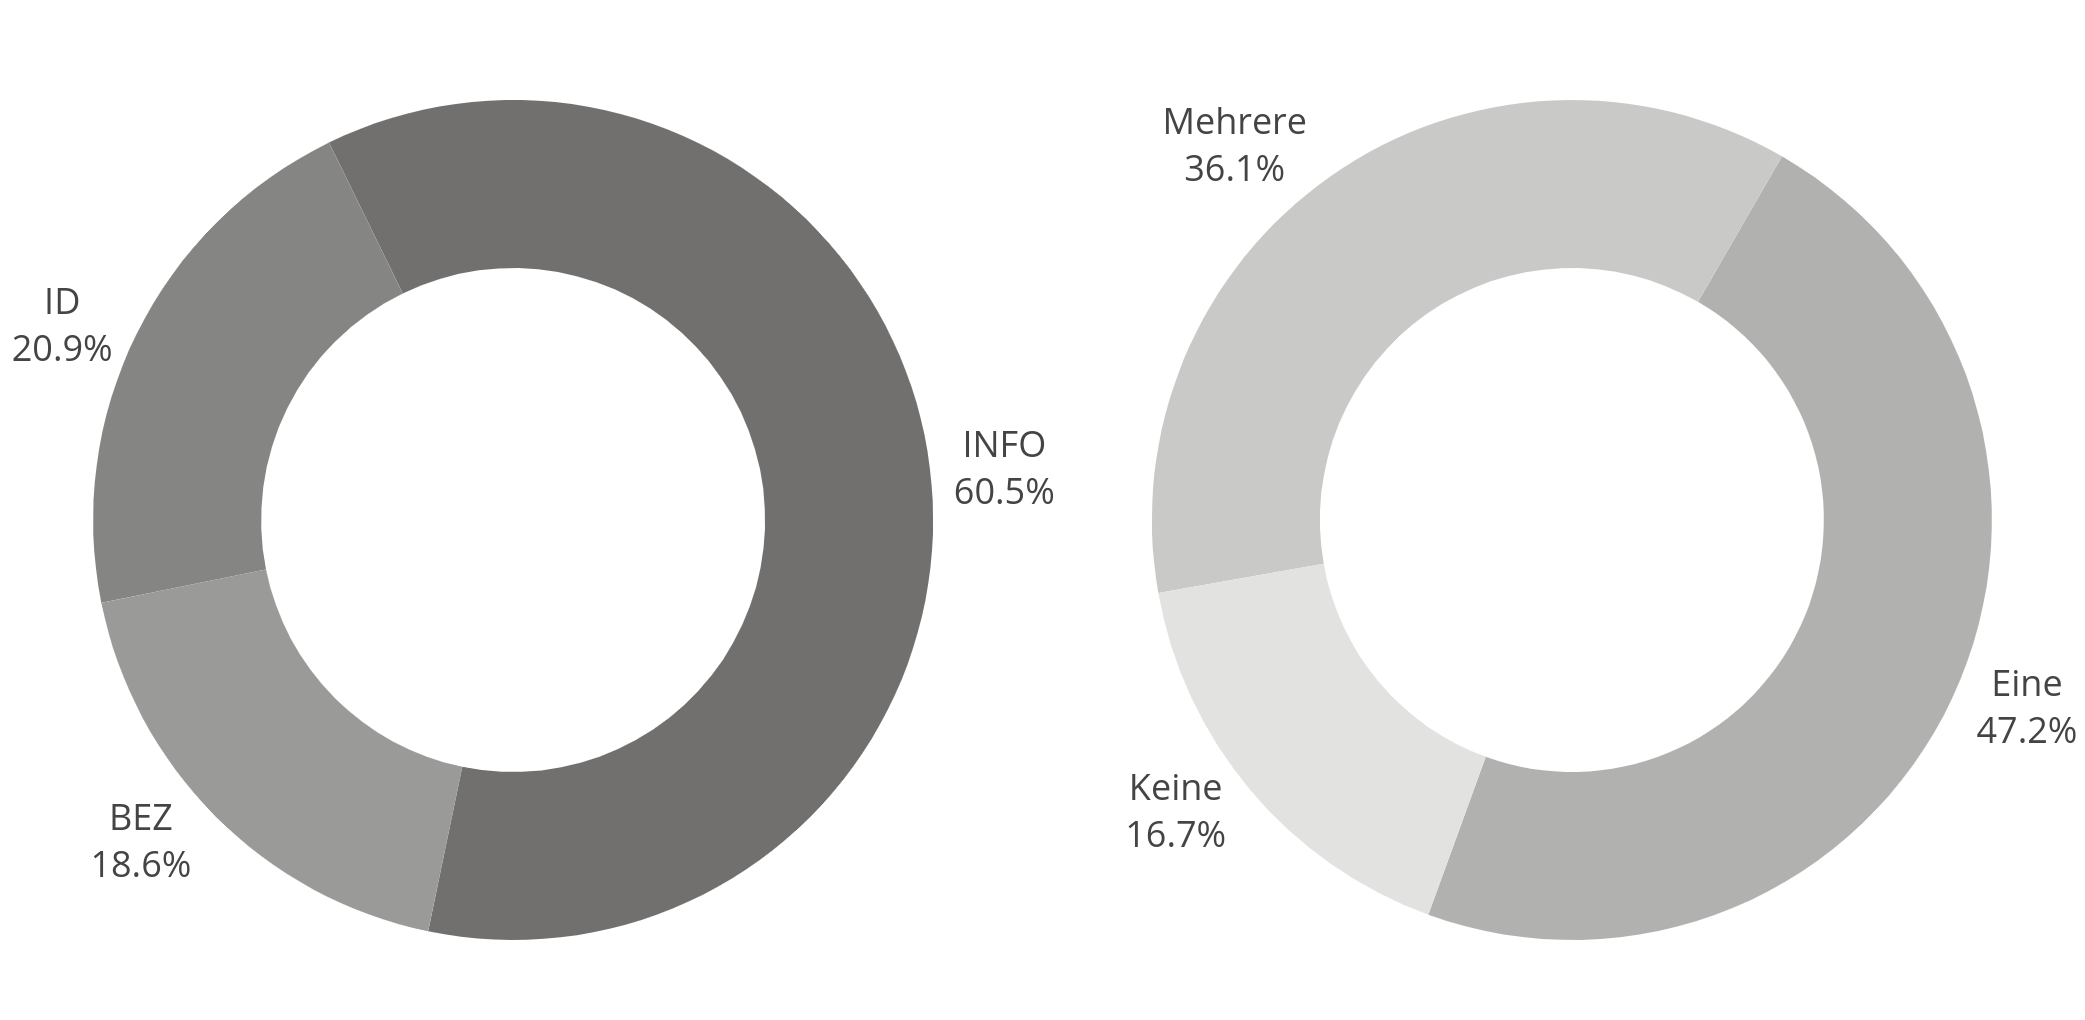
\includegraphics[width=.9\textwidth]{img/plots/kat/kat_fb.png}
    \caption{Prozentuale Verteilung der Facebook-Beiträge in die Management-Leistungen nach Jan-Hinrik Schmidt. Links die Kategorisierung nach Management-Leistungen, rechts die Angabe, wie häufig Zuteilungen zu Management-Leistungen gemacht werden konnten.}
    \label{fig:kategoriefb}
\end{figure}  

\subsubsection{Blog}

Tabelle \ref{tab:kategoriebl} zeigt die Einteilung der Blog-Beiträge der Universität Bielefeld im Juli 2018 in die in \ref{sec:jhsforschung} eingeführten Management-Leistungen. Wie (auch in Abbildung \ref{fig:kategoriebl}) zu sehen ist, sind alle Beiträge des Blogs mindestens der Kategorie Informationsmanagement zugeordnet. Ein Beitrag kann zusätzlich dem Beziehungsmanagement zugeordnet werden. Wie die Abbildung \ref{fig:kategoriebl} zeigt, handelt es sich dabei um einen Anteil von 2.17 \% an der Gesamtheit der Blog-Beiträge. 34.8 \% der Beiträge wurden neben dem Informationsmanagement auch dem Identitätsmanagement zugeordnet. Der rechte Teil der Abbildung \ref{fig:kategoriebl} zeigt außerdem die ausgeglichene Verteilung von Einfach- und Mehrfachzuordnungen in die Management-Leistungen.

\begin{table}[H]
    \caption{Blog Beiträge der Universität Bielefeld im Juli 2018 und ihre Zuordnung zu den Management-Leistungen nach Schmidt.}
\resizebox{\textwidth}{!}{%
\begin{tabular}{*{29}{c|}c}
 & \rotatebox{270}{BL\_02\_01 } & \rotatebox{270}{BL\_02\_02} & \rotatebox{270}{BL\_02\_03} & \rotatebox{270}{BL\_03\_01} & \rotatebox{270}{BL\_04\_01} & \rotatebox{270}{BL\_04\_02} & \rotatebox{270}{BL\_05\_01} & \rotatebox{270}{BL\_05\_02} & \rotatebox{270}{BL\_05\_03} & \rotatebox{270}{BL\_06\_01} & \rotatebox{270}{BL\_10\_01} & \rotatebox{270}{BL\_10\_02} & \rotatebox{270}{BL\_11\_01} & \rotatebox{270}{BL\_12\_01} & \rotatebox{270}{BL\_13\_01} & \rotatebox{270}{BL\_16\_01} & \rotatebox{270}{BL\_16\_02} & \rotatebox{270}{BL\_17\_01} & \rotatebox{270}{BL\_17\_02} & \rotatebox{270}{BL\_18\_01} & \rotatebox{270}{BL\_20\_01} & \rotatebox{270}{BL\_24\_01} & \rotatebox{270}{BL\_25\_01} & \rotatebox{270}{BL\_26\_01} & \rotatebox{270}{BL\_26\_02} & \rotatebox{270}{BL\_27\_01} & \rotatebox{270}{BL\_30\_01} & \rotatebox{270}{BL\_30\_02} & \rotatebox{270}{BL\_31\_01} \\
 \hline
ID &  & X & X & X & X &  &  & X & X & X &  &  & X &  &  & X &  &  & X &  &  & X & X & X &  & X & X &  & X \\
\hline
BEZ &  &  &  &  &  &  &  &  &  &  &  &  &  &  &  &  &  &  &  &  &  &  &  &  & X &  &  &  &  \\
\hline
INFO & X & X & X & X & X & X & X & X & X & X & X & X & X & X & X & X & X & X & X & X & X & X & X & X & X & X & X & X & X
\end{tabular}%
}
\label{tab:kategoriebl}
\end{table}

\begin{figure}[H]
    \centering
    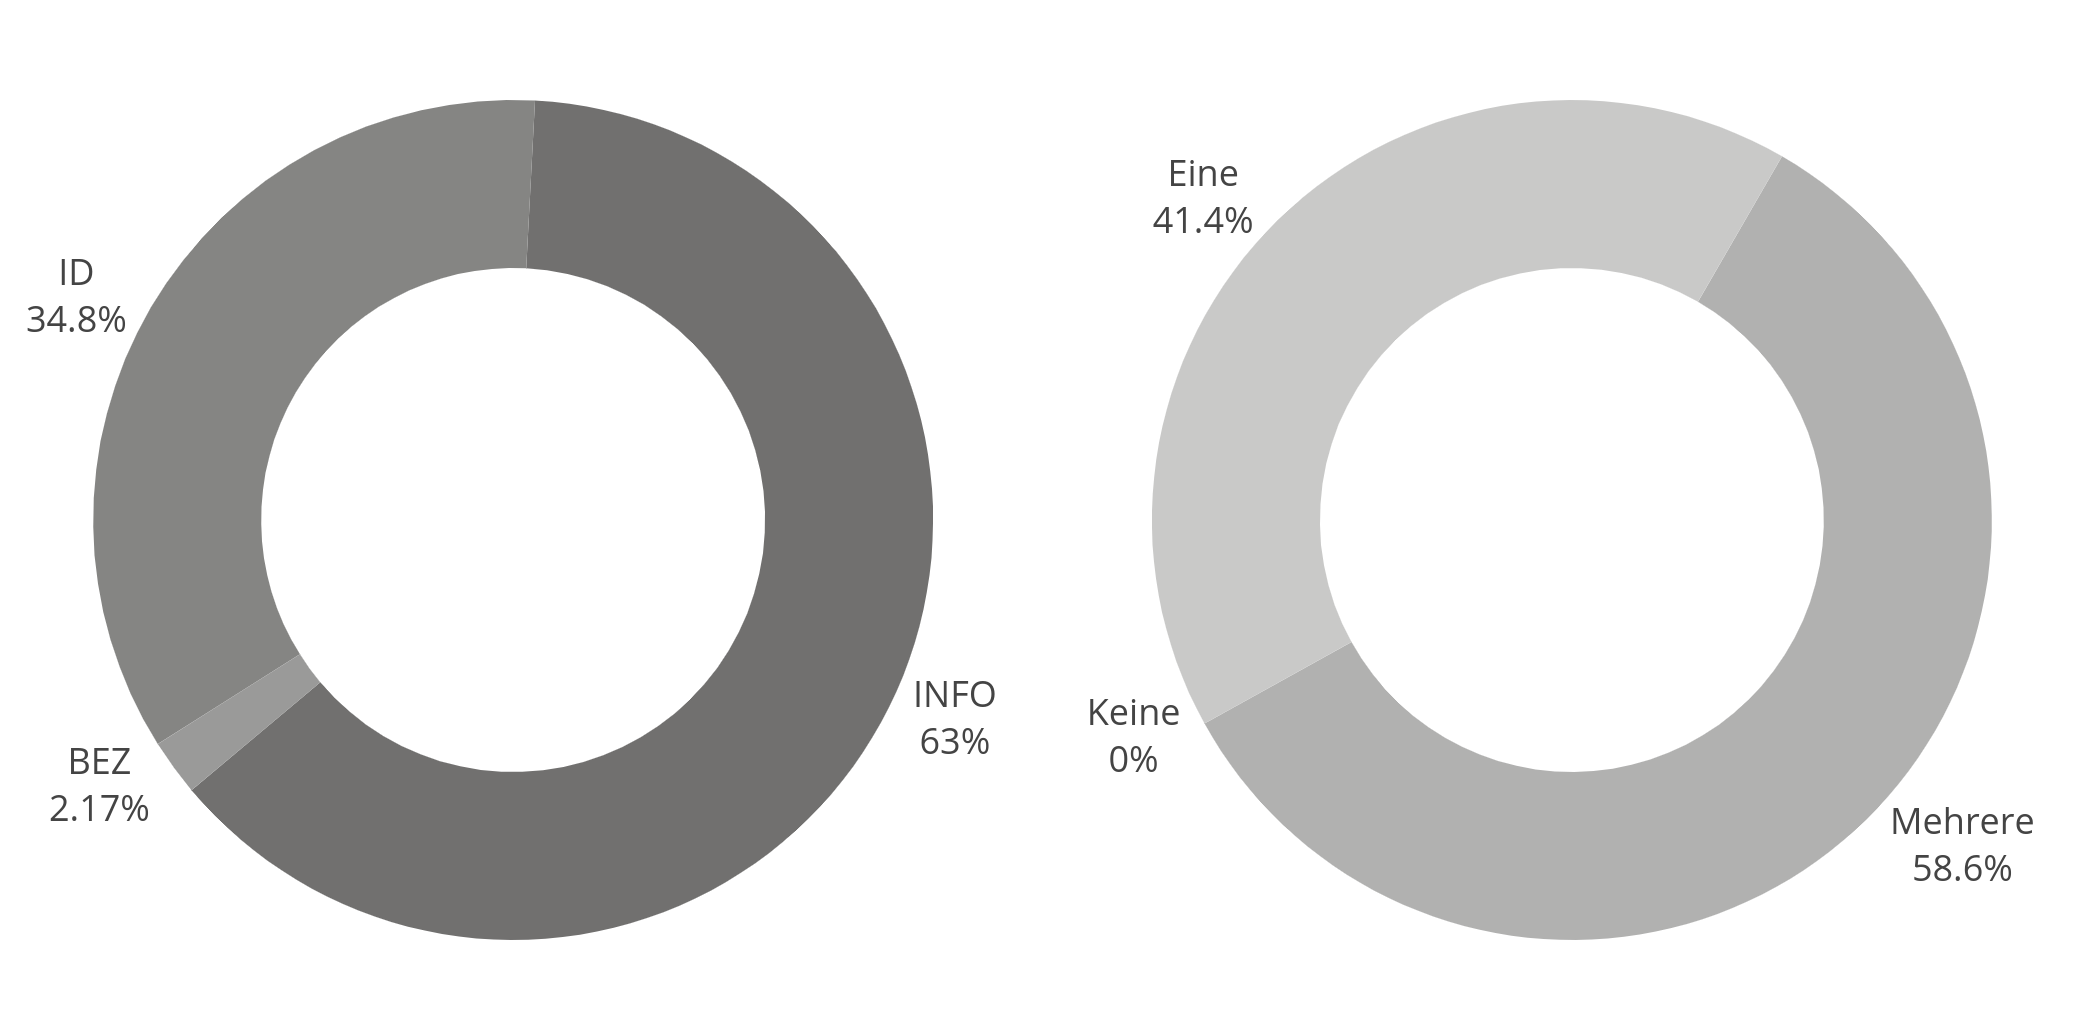
\includegraphics[width=.9\textwidth]{img/plots/kat/kat_bl.png}
    \caption{Prozentuale Verteilung der Blog-Beiträge in die Management-Leistungen nach Jan-Hinrik Schmidt. Links die Kategorisierung nach Management-Leistungen, rechts die Angabe, wie häufig Zuteilungen zu Management-Leistungen gemacht werden konnten.}
    \label{fig:kategoriebl}
\end{figure}  

\subsubsection{Twitter}

Wie in Tabelle \ref{tab:kategorietw} zu sehen ist, wurde Twitter im untersuchten Monat nicht zum Beziehungsmanagement verwendet. Sechs von sieben Beiträgen auf Twitter folgen dem Informationsmanagement, vier dem Identitätsmanagement. Ein Beitrag ist keiner der Kategorien zuzuordnen. Wie in den oberen Abschnitten über Facebook und den Universitäts-Blog auch, lassen sich in der hier aufgezeigten Abbildung \ref{fig:kategorietw} die Aufteilungen in die Management-Leistungen ablesen. 

\begin{table}[h]
    \caption{Blog Beiträge der Universität Bielefeld im Juli 2018 und ihre Zuordnung zu den Management-Leistungen nach Schmidt.}
\resizebox{\textwidth}{!}{%
\begin{tabular}{*{7}{c|}c}
 & TW\_03\_01 & TW\_10\_01 & TW\_11\_01 & TW\_13\_01 & TW\_25\_01 & TW\_27\_01 & TW\_30\_01 \\
 \hline
ID & X &  & X &  & X & X &  \\
\hline
BEZ &  &  &  &  &  &  &  \\
\hline
INFO & X & X & X & X & X & X & 
\end{tabular}%
}
\label{tab:kategorietw}
\end{table}

\begin{figure}[h]
    \centering
    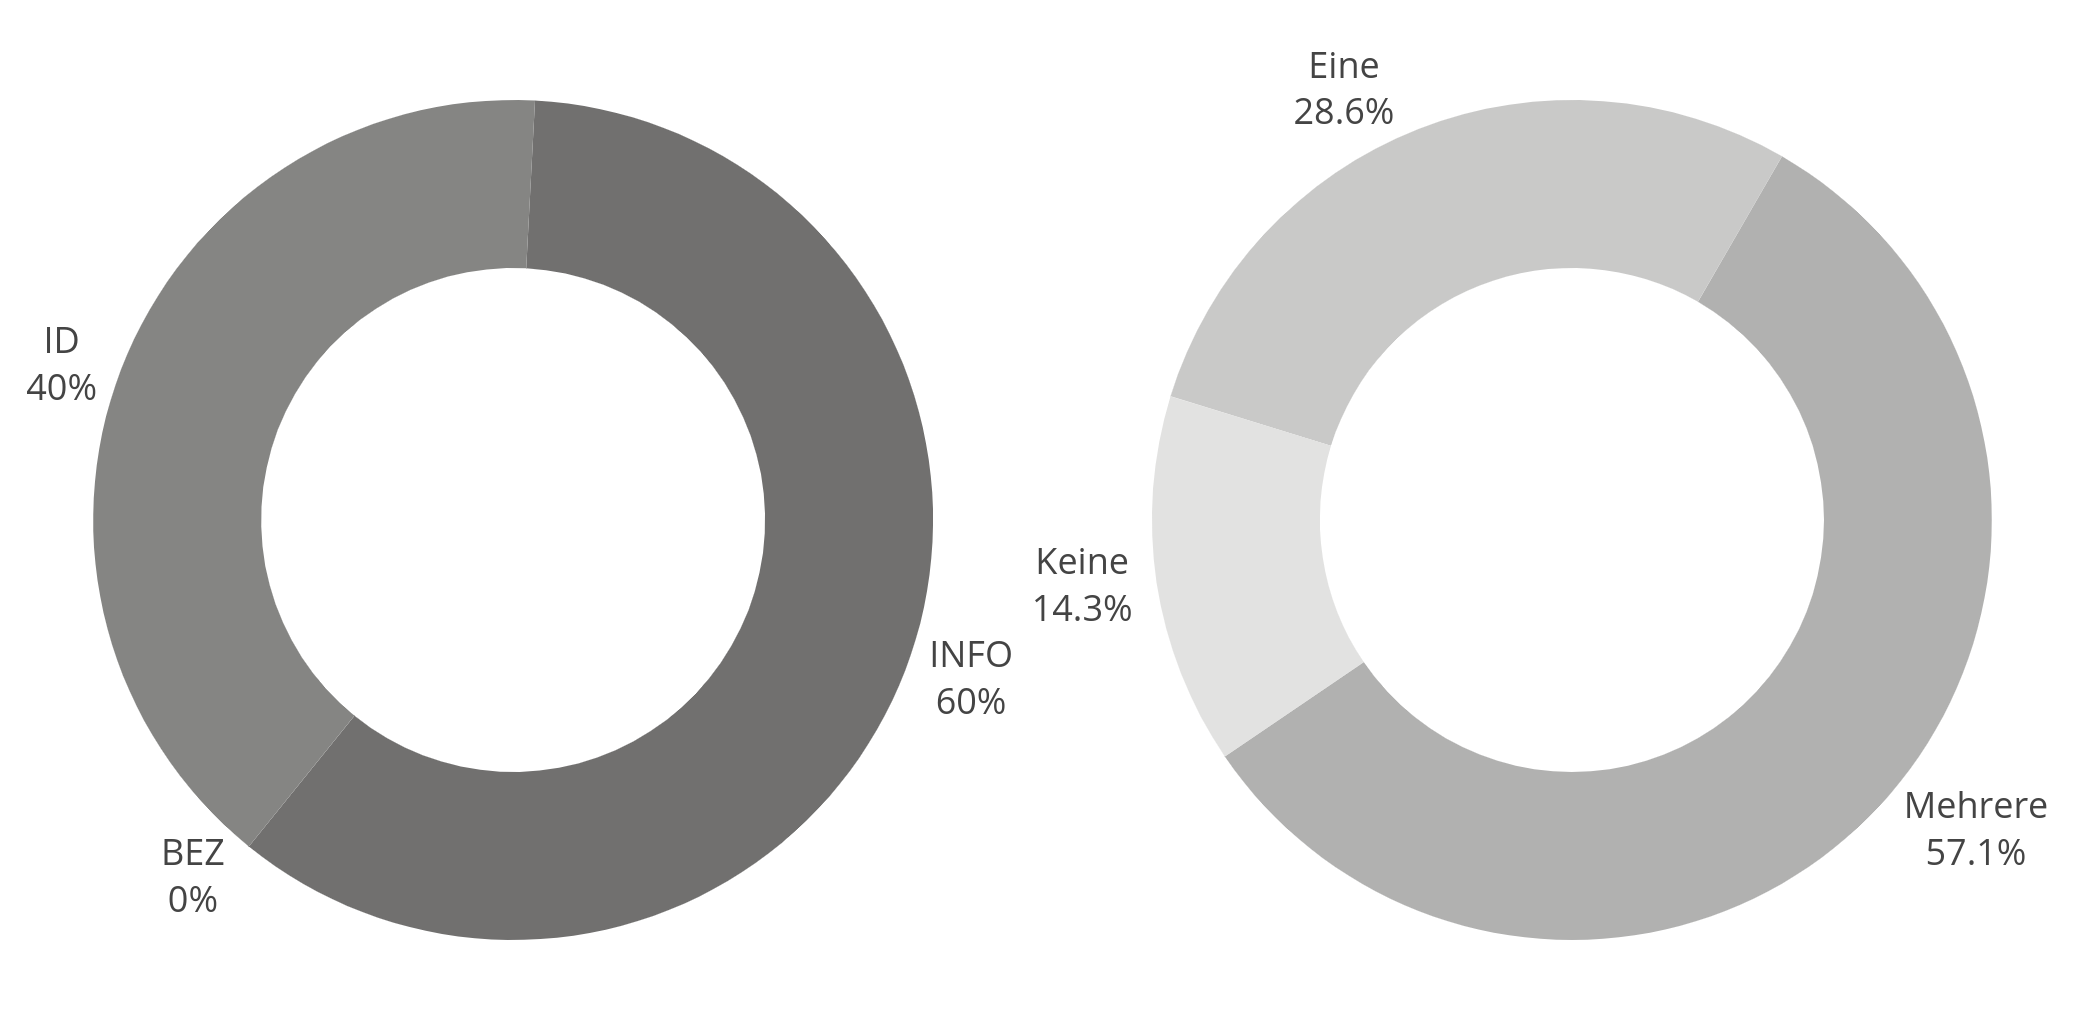
\includegraphics[width=.9\textwidth]{img/plots/kat/kat_tw.png}
    \caption{Prozentuale Verteilung der Twitter-Beiträge in die Management-Leistungen nach Jan-Hinrik Schmidt. Links die Kategorisierung nach Management-Leistungen, rechts die Angabe, wie häufig Zuteilungen zu Management-Leistungen gemacht werden konnten.}
    \label{fig:kategorietw}
\end{figure}  

\section{Ergebnisse}
\label{sec:Ergebnisse}

% Darstellung der Auswertung der Daten. Hier wird nicht interpretiert. Es werden nicht die Hypothesen beantwortet. - beschreibende Daten

Tabelle \ref{tab:socialmediapostsprozent} zeigt, dass mit 36 Beiträgen, Facebook \printpercent{36}{105} aller Beiträge ausmacht. Twitter ist mit sieben Beiträgen, und damit \printpercent{7}{105}, der im Juli 2018 am wenigsten genutzte Social Web Kanal der Universität. YouTube-Videos machen \printpercent{11}{105}, Instagram-Beiträge \printpercent{22}{105}, und Blog-Beiträge \printpercent{29}{105} der Social Web Beiträge aus.

\begin{table}[H]
    \centering
    \caption{Prozentuale Verteilung der Social Web Beiträge der Universität Bielefeld im Juli 2018.}
        \begin{tabular}{*{5}{l}}
        Facebook & Universitäts-Blog & Instagram & YouTube & Twitter \\
        \hline
        \printpercent{36}{105} & \printpercent{29}{105} & \printpercent{22}{105} & \printpercent{11}{105} & \printpercent{7}{105}
    \end{tabular}
    \label{tab:socialmediapostsprozent}
\end{table}

Im Gegensatz zu der relativ eindeutigen Follower-Verteilung (Abbildung \hyperref[fig:follower]{\ref{fig:follower} \& Tabelle \ref{tab:followerprozent}}), die einen starken Überhang an Facebook-Followern gegenüber allen anderen Plattformen zeigt, sind die Beiträge -- mit Ausnahme der Twitter-Beiträge -- eher gleichmäßig verteilt.

Von den 105 Beiträgen, die die Universität im Juli über alle Plattformen veröffentlicht hat, wurden in Abschnitt \ref{sec:jhseinteilung} die auf Text basierten 72 Beiträge der Plattformen Facebook, Twitter und Universitäts-Blog untersucht und kategorisiert. Von den 72 untersuchten Beiträgen konnten, wie in Abbildung \ref{fig:kategorietext} zu sehen, 43.1 \% der Beiträge eindeutig einer Kategorie zugeordnet werden. Bei etwa 47 \% der Beiträge ließen sich zwei oder sogar drei Kategorien zuteilen. Fast 10 \% aller Beiträge konnten jedoch keiner der drei Management-Leistungen uneingeschränkt zugewiesen werden.

\begin{figure}[H]
    \centering
    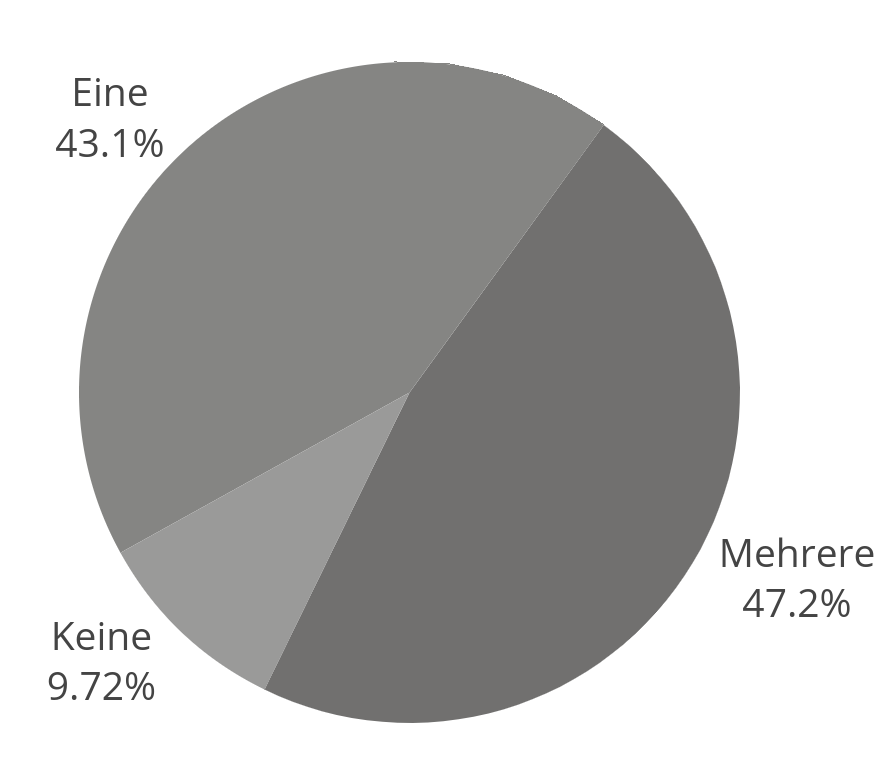
\includegraphics[width=.5\textwidth]{img/plots/kat/kat_text.png}
    \caption{Prozentuale Verteilung der Zuordnungshäufigkeit der auf Text basierten Social Web Beiträge in die Management-Leistungen. Der Datensatz umfasst 72 Beiträge.}
    \label{fig:kategorietext}
\end{figure}  

Abbildung \ref{fig:kategorietextprozent} zeigt, dass der Großteil der Beiträge im Kern Informationsbeiträge gewesen sind. Knapp 72 \% aller Facebook-, über 85 \% aller Twitter- und ohne Ausnahme alle Blog-Beiträge konnten mit dem Informationsmanagement kategorisiert werden. Der Anteil an Beziehungsmanagement ist bei Facebook mit 22.22 \% am höchsten. Nur 3.45 \% des Blog-Beiträge haben -- zum Beispiel durch den Aufruf zu Mitarbeiten, Veranstaltungen, und Ähnlichem -- Beziehungsmanagement betrieben. Bei den Twitter-Beiträgen im Juli konnte kein Beitrag dieser Kategorie zugeordnet werden. Dem Identitätsmanagement konnten von den Facebook-Beiträgen ein Viertel, und mit jeweils 55.17 \% und 57.14 \% knapp über die Hälfte der Blog- und Twitter-Beiträge zugeordnet werden.

\begin{figure}[h]
    \centering
    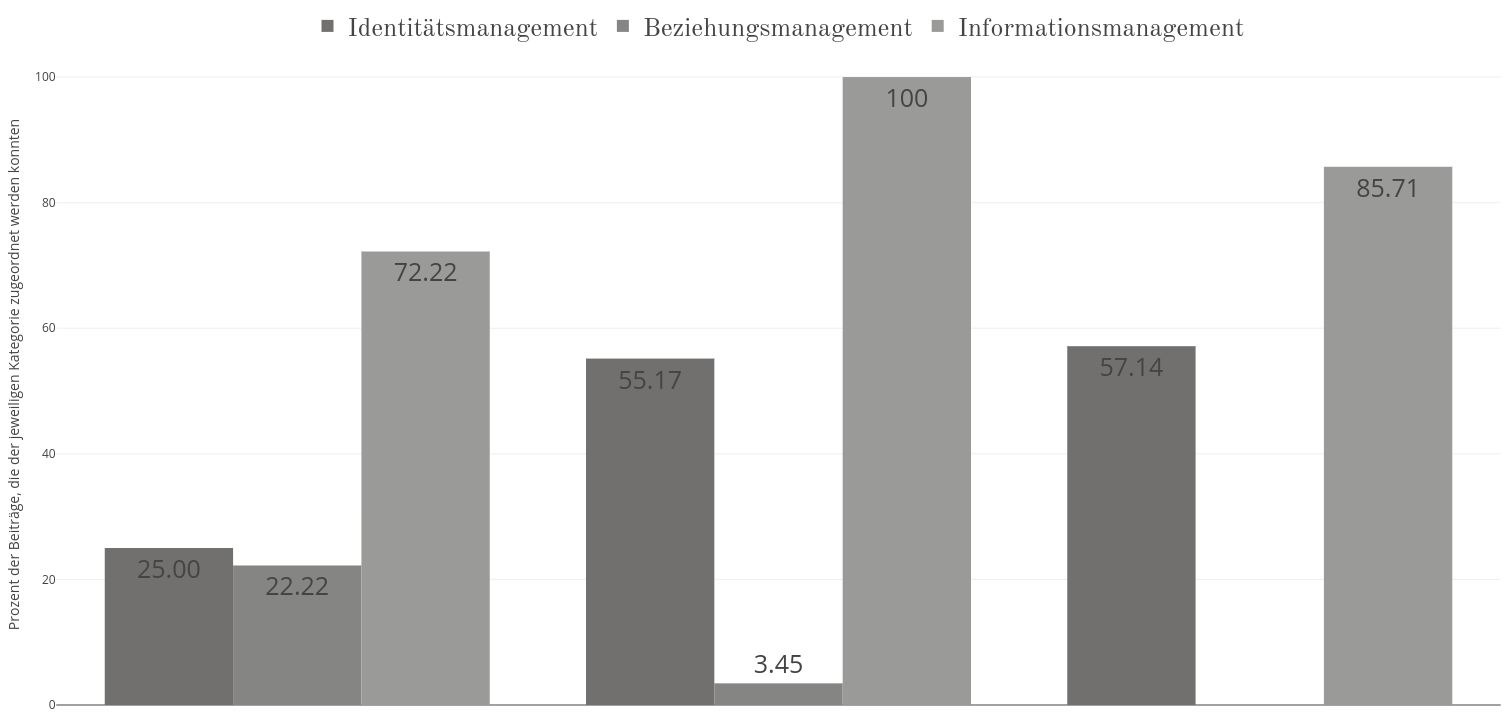
\includegraphics[width=\textwidth]{img/plots/kat/kat_text_prozent.png}
    \caption{Prozentuale Verteilung der Zuordnungshäufigkeit der auf Text basierten Social Web Beiträge in die Management-Leistungen. Der Datensatz umfasst 72 Beiträge. Der linke Teilgraph zeigt Facebook-Beiträge, der mittlere Blog-Beiträge und der rechte Twitter-Beiträge.}
    \label{fig:kategorietextprozent}
\end{figure} 

\section{Diskussion}
\label{sec:Diskussion}

% Zusammenfassung der Ergebnisse - Hypothesen bestätigt? Falsifiziert? (Bewertung) - Fragestellung geklärt? - Theoriebedeutung - Kurze Praxisbedeutung - Kritische Diskussion der Ergebnisse - Mängel / Verbesserungen der Studie

Mit der stetig wachsenden Nutzung von Social Web Plattformen, machen immer häufiger auch Firmen, Vereine und Institutionen Gebrauch vom Potenzial der einfachen Erreichbarkeit über das Internet; ob für die Wertsteigerung des Unternehmens oder im Personalmanagement (vgl. \cite{culnan2010large} \& \cite{barmann2016social}). Schaut man sich die größten Universitäten des Landes an, haben alle bis auf sehr wenige Ausnahmen mindestens dasselbe Social Web Repertoire, wie die Universität Bielefeld. Herausstechen tut die Universität Duisburg Essen, die zusätzlich dazu noch Snapchat, Google+, Flickr, XING, LinkedIn und sogar eine eigene Campus-App bereitstellt\footnote{Universität Duisburg-Essen -- \url{https://www.uni-due.de/}}. Das Angebot der verschiedenen Social Web Plattformen steigt -- wie man an der Universität Duisburg-Essen gut sieht -- immer weiter, weshalb sich gerade Institutionen, die sich nur eine durch das Personal eingeschränkte Bespeisung der Netzwerke leisten können, im Normalfall auf einige wenige Plattformen beschränken müssen. Die Universität Bielefeld hat auf den verschiedenen Social Web Plattformen insgesamt 34.140 Follower. Davon fallen knapp die Hälfte Facebook zu. Knapp 7.000 Nutzerinnen und Nutzer folgen der Universität Bielefeld auf Instagram, und etwas über 6.000 Follower kann der Universitäts-Twitter-Account verzeichnen. Den YouTube-Kanal der Universität abonnierten, Stand September 2018, nur 800 Personen. Diese 34.140 Follower werden von sechs Mitarbeiterinnen und Mitarbeitern der Universität unterhalten\footnote{\href{https://ekvv.uni-bielefeld.de/pers_publ/publ/EinrichtungDetail.jsp?orgId=7116054}{Abteilung \textit{Medien und News}, Referat für Kommunikation}}.

Die Analyse des vorliegenden Datensatzes der Social Web Beiträge der Universität Bielefeld aus dem Juli 2018 ergab, dass auch hier eine begründete Selektion stattfand. 72 der 105 untersuchten Beiträge wurden auf im Kern textbasierten Social Web Plattformen veröffentlicht. YouTube-Videos und Instagram-Bilder und -Videos stellen den etwas kleineren Teil der Beiträge dar und wurden für die inhaltliche Analyse mithilfe der Forschungen von Jan-Hinrik Schmidt (siehe \ref{sec:jhsforschung}) außer Acht gelassen.

Die 72 näher untersuchten Beiträge teilen sich in 50 \% Facebook-Beiträge, etwa 40 \% Blog-Beiträge und etwa 10 \% Twitter-Beiträge auf. Die 50 \% Facebook-Beiträge korrelieren hier sehr stark mit den oben genannten Follower-Zahlen. Bei allen anderen Plattformen ist eine solche Korrelation jedoch nicht erkennbar. Die etwas über 6.000 Twitter-Follower wurden in dem untersuchten Monat nur mit sieben Beiträgen beglückt, die sich teilweise auch mit Beiträgen der anderen Plattformen doppeln. Der YouTube-Kanal hat hingegen mit $1:72$ die höchste Rate von Beiträgen zu Abonnenten. Dies könnte damit erklärt werden, dass in der Gesamtheit die Zahl der YouTube-Videos weit unter der Zahl der Beiträge auf den anderen Social Web Plattformen liegt, und deshalb (noch) nicht viele Nutzerinnen und Nutzer von dem Kanal wissen oder regelmäßig die Videos schauen. Zudem ist die soziale Hürde einen YouTube-Kanal zu abonnieren, höher als die, eine Seite auf Facebook mit einem Like zu markieren. Zu den wenigen Abonnenten kommen dann in letzter Zeit  immer mehr Video-Beiträge, unter anderem durch Universitäts-Formate wie \textit{Campus TV}\footnote{Campus TV Universität Bielefeld -- \url{https://lul.uni-bielefeld.de/projekte/campustv}} oder das Seminar \textit{Vosicht Podcast!}, welches seit 2008\footnote{\href{https://uni-bielefeld.de/kvv_publ/publ/Lehrende_Veranstaltungen.jsp?personId=3772740}{Paul John -- Vorsicht Podcast!}} regelmäßig für verschiedenste Studiengänge angeboten wird.


Bei der Einordnung der Beiträge zu den Management-Leistungen der Social Web Anwendungen konnte gezeigt werden, dass 90 \% der Beiträge mindestens einer Leistung zugewiesen werden können. Bei knapp 10 \% der Beiträge war eine solche Zuordnung jedoch nicht möglich. Dies ist ein überaus signifikanter Teil der Beiträge. Die Fragestellungen aus Kapitel \ref{sec:hypothesen}, ob das Modell nach Jan-Hinrik Schmidt auf die Social Web Kommunikation der Universität Bielefeld anwendbar ist, und die Beiträge der Universität, wie die einer Einzelperson, in die drei Management-Leistungen Identitätsmanagement, Beziehungsmanagement und Informationsmanagement eindeutig zugeordnet werden können, müssen demnach beide verneint werden. 

Außerdem kann aus den Ergebnissen hergeleitet werden, dass die ebenfalls in Kapitel \ref{sec:hypothesen} erarbeitete Hypothese dieser Abschlussarbeit bestätigt werden kann. Das untersuchte Modell kann nach jetzigem Stand nicht ohne Überarbeitung auf die Social Web Kommunikation von Institutionen angewandt werden.

Dadurch, dass es sich um die Anwendung eines etablierten Modells auf einen Bereich handelt, der von dem Modell nicht intendiert gewesen ist, handelt es sich bei dem Ergebnis nicht um eine Kritik am Modell nach Jan-Hinrik Schmidt, sondern um die Feststellung, dass sich die Social Web Kommunikation einer Einzelperson von der einer Institution so weit unterscheidet, dass das Modell dort unüberarbeitet keine Anwendung finden kann.

Zuletzt möchte ich in diesem Kapitel -- trotz der Bestätigung der Arbeitshypothese -- kritisch auf den Aufbau der Arbeit schauen und Möglichkeiten aufzeigen, wie sich die Arbeit verbessern ließe. Zur Ermöglichung der Verarbeitung, wurde der untersuchte Datensatz auf einen Monat beschränkt. Auch wenn der Zeitraum in Abschnitt \ref{sec:Datenauswahl} begründet wurde, so bleibt dennoch die Frage nach der Repräsentativität des Datensatzes. Durch die händische Verarbeitung musste der Datensatz stark limitiert werden. Ein größerer Datensatz, beispielsweise über einen Zeitraum von einem ganzen Semester, würde repräsentativere Daten ergeben, und ermöglichen, eine bessere Einschätzung bekommen zu können, ob die Modell-Anwendbarkeit gegeben ist oder nicht. 
Im Rahmen dieser Arbeit wurden außerdem nur die textbasierten Social Web Plattformen untersucht; die visuell ausgerichteten Foto- und Video-Plattformen -- namentlich Instagram und YouTube -- wurden außer Acht gelassen. Dadurch gehen ebenfalls Daten verloren, die die Analyse und somit das Ergebnis der Arbeit beeinflussen hätten können. Eine händische Kategorisierung ist außerdem Fehlerbehaftet, da sie im Zweifelsfall nicht stark genug fixierten Regeln folgt. Die Aussagekraft der Einordnung in Kategorien in Abschnitt \ref{sec:jhseinteilung} ist demnach nicht fest reguliert und daher womöglich nicht aussagekräftig genug. 
Des Weiteren war die Datenauswahl auf Ursprungs-Beitrags-Daten beschränkt. Dies meint, dass Die Nutzerinnen- und Nutzer-Interaktionen, wie das Liken von Facebook-Beiträgen, das Retweeten von Twitter-Beiträgen und das Kommentieren im Allgemeinen nicht analysiert wurden und somit womöglich der Aspekt des Beziehungsmanagements nicht hinreichend bearbeitet wurde.

Die oben angesprochenen visuellen Plattformen aus der Analyse raus zu lassen, hatte im Rahmen dieser Arbeit den Umfang betreffende Praktikabilitätsgründe. Die Daten, die im Zuge dessen verloren gehen, ließen sich durch die Nutzung der von YouTube automatisch generierten Untertitel, oder, da diese recht ungenau sind (vgl. \cite{parton2016video}), durch vorherige Annotationsarbeiten wiederum verwendbar machen.  Dazu könnten beispielsweise Skripte der YouTube-Videos erstellt, oder auch die Instagram-Fotos mithilfe digitaler Bilderkennungssoftware verschlagwortet werden. Um den oben genannten Kritikpunkten an der Arbeit entgegen zu kommen, böte sich außerdem an, die Verarbeitung der Daten zu automatisieren. Damit ließe sich zum einen die Datenanalyse skalieren, bis hin zur Verarbeitung aller öffentlich zugänglichen Social Web Beiträge, und zum anderen auch die oben angesprochenen Annotationen der Bilder und Videos in die Datenverarbeitung mit einbeziehen.

Eine solche Automatisierung könnte dann über programmatisch festgelegte Kategorisierungsregeln oder mithilfe der Verarbeitung von großen Datenmengen mittels künstlicher Intelligenz und neuronaler Netzwerke erfolgen. Solch große Datenmengen würden dann die Repräsentativität der Analyseergebnisse nochmals verbessern können.
\chapter{Fazit und Ausblick}
\label{chap:Fazit}

% Ergebnisse zusammenfassen und bewerten - Beantworten der Fragen aus der Einleitung - Ausblick / Offene Fragen / Angrenzende Themengebiete
% KEINE neuen Erkenntnisse / Thesen

Die Ergebnisse aus Kapitel \ref{sec:Ergebnisse} zeigen, dass nicht für alle Beiträge eine Kategorisierung möglich ist, wie sie Schmidt für die Social Web Kommunikation postuliert. 10 \% der analysierten Social Web Beiträge der Universität aus dem Juli 2018 haben sich nicht in dem Modell widerspiegeln lassen.

In der Annahme, dass das Modell der Management-Leistungen nach Jan-Hinrik Schmidt aus Abschnitt \ref{sec:jhsforschung} eine Kategorisierung aller veröffentlichter Beiträge im Social Web garantiert, ist eine vollständige Übernahme des Modells von der persönlichen auf die Institutions-Kommunikation im Social Web daher nicht möglich. 

Die kritische Begutachtung der Arbeit in Kapitel \ref{sec:Diskussion} zeigt, dass eine weniger kommunikationswissenschaftliche -- sondern im Kern computerlinguistische -- Arbeit zu repräsentativeren Ergebnissen kommen könnte. Eine solche technischer ausgelegte Arbeit könnte dann den Rahmen des Datensatzes erweitern oder gar aufheben. Sie könnte Social Web Beiträge dem Inhalt nach automatisiert analysieren. Die Beschaffung der Daten kann vollständig automatisiert über die APIs (Application Programming Interfaces -- Programmierschnittstellen) der jeweiligen Social Web Plattformen erfolgen. Für die inhaltliche Verarbeitung kommen diverse Techniken des NLP (Natural Language Processing) zum Einsatz. Eine simple Technik wäre das sogenannte TF/IDF (Term Frequency/ Inverse Document Frequency), welches durch die Berechnung der Häufigkeiten von im Text vorkommenden Begriffen, in der Lage ist, Themenbereiche eines Textes herauszufinden und so Social Web Beiträge automatisiert verschlagworten könnte (vgl. \cite{ramos2003tfidf}). Ramos selber bedient sich in seiner Arbeit weiteren computerlinguistischen Techniken, die sich unter anderem in \cite{kiss2006unsupervised}, \cite{mitkov2012coreference} und \cite{uryupina2006coreference} wiederfinden. Diese Techniken des NLP finden unter anderem Anwendung in der automatischen Textzusammenfassung. Das Zwischenziel der automatisierten Textzusammenfassung ist es, den Inhalt eines Textes programmatisch zu erfassen. Dies kann dazu genutzt werden, die Social Web Beiträge in die Kategorien des Modells von Jan-Hinrik Schmidt einzuteilen.

Gelingt eine solche Vollautomatisierung des Prozesses, können schier endlose Datenmengen in kürzester Zeit analysiert, und daraus signifikant relevante Ergebnisse abgeleitet werden, wie es \textit{per Hand} nicht machbar wäre.


%% ---------------------------------------%%

%\pagestyle{plain}

\addtocontents{toc}{\vspace{\normalbaselineskip}}
\addtocontents{toc}{\hrule}
\addtocontents{toc}{\vspace{\normalbaselineskip}}

\pagenumbering{Roman}
\bibliographystyle{apalike}
\bibliography{ba_thesis.bib}

\clearpage
\addcontentsline{toc}{chapter}{Eigenständigkeitserklärung}
\begin{doublespace}
\newgeometry{left=2.5cm,right=2.5cm,top=2cm,bottom=2cm}
%\doublespacing

{\let\clearpage\relax \chapter*{\centerline{Eigenständigkeitserklärung}}}
\label{chap:Erklärung}

\vspace*{1cm}

\setlength{\parindent}{0pt}
Hiermit erkläre ich, dass ich die vorliegende Bachelorarbeit eigenständig verfasst, und gelieferte Datensätze, Zeichnungen, Skizzen und graphische Darstellungen eigenständig erstellt habe. Ich habe keine anderen Quellen als die angegebenen benutzt und habe die Stellen der Arbeit, die anderen Werken entnommen sind - einschließlich verwendeter Tabellen und Abbildungen - in jedem einzelnen Fall unter Angabe der Quelle als Entlehnung kenntlich gemacht.

\vspace*{2cm}

Bielefeld, den \today \hfill \hrulefill

\hspace*{0mm}\phantom{Bielefeld, den} 
\hfill Fabian Wohlgemuth\hspace*{1cm}
\restoregeometry
\end{doublespace}

\addcontentsline{toc}{chapter}{Anhang}
\chapter*{Anhang}
\label{chap:Anhang}

\section*{Social Media Posts}

\begin{figure}[h]
    \centering
    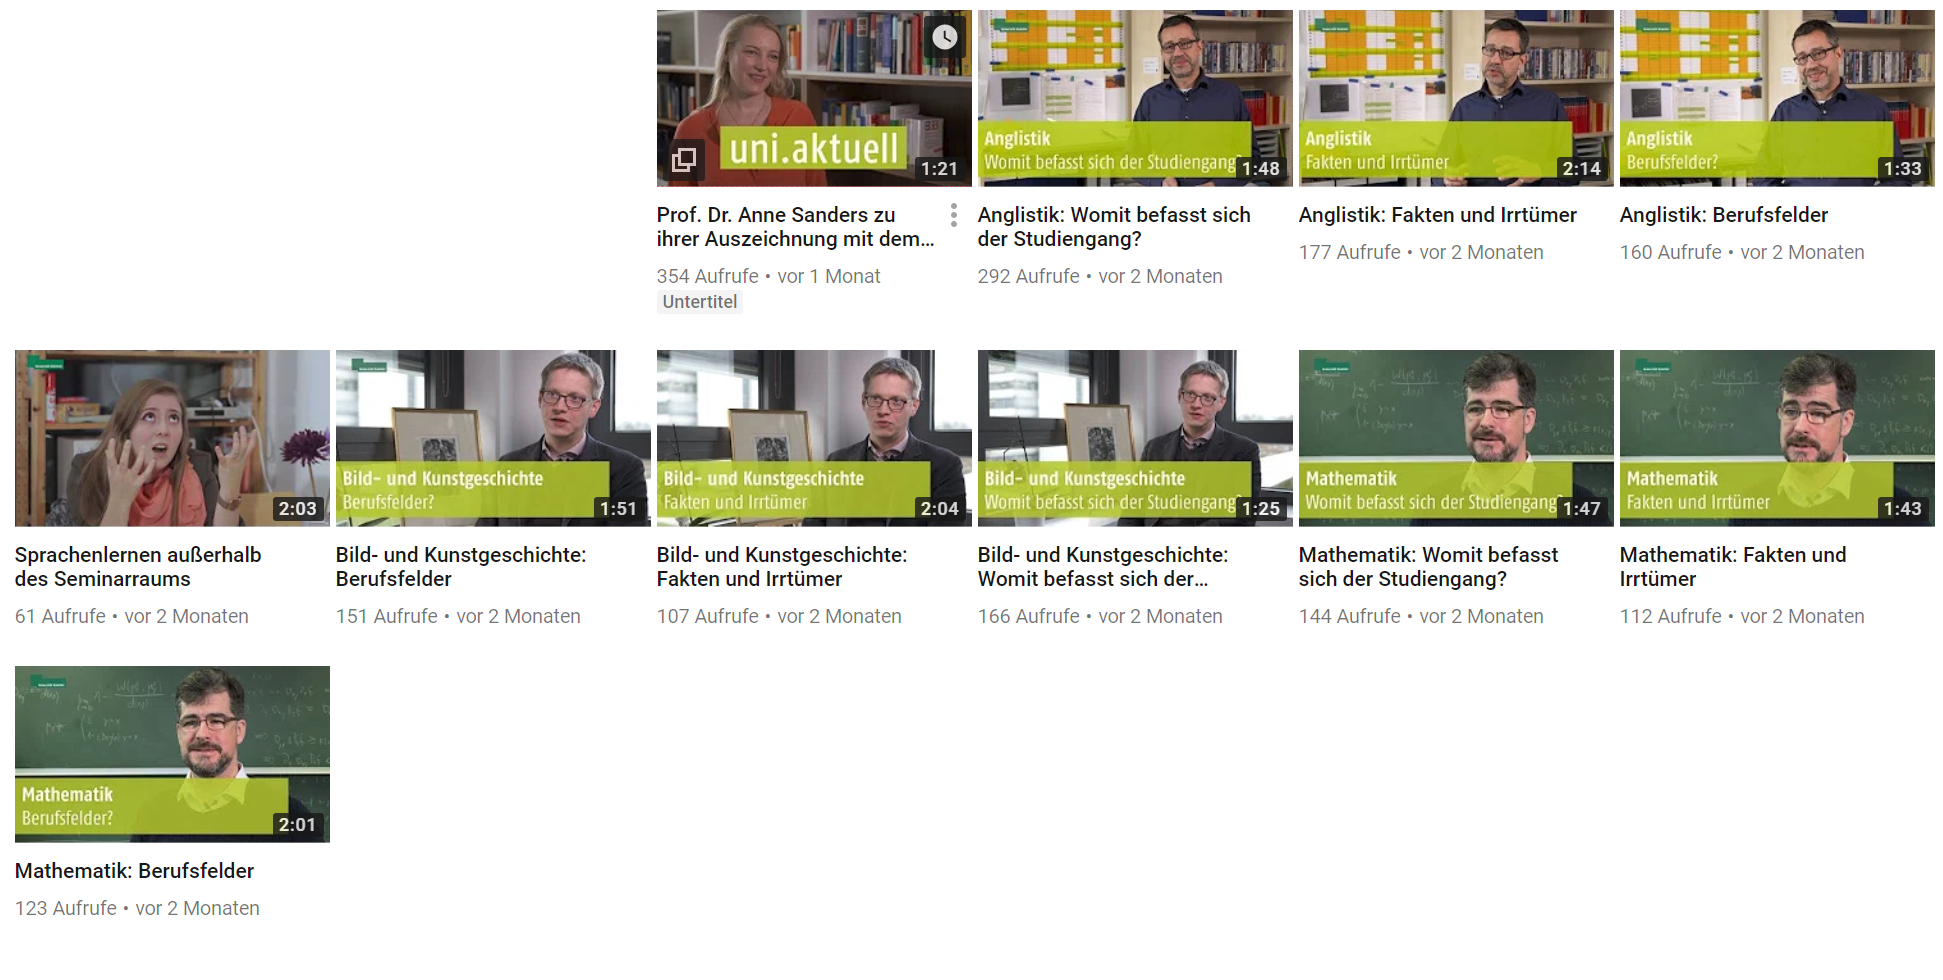
\includegraphics[width=1.2\textwidth]{img/posts/yt.png}}
    \caption{YouTube Posts - Universität Bielefeld - Juli 2018 \newline \href{https://www.youtube.com/user/bielefelduniversity/videos}{youtube.com/user/bielefelduniversity/videos}}
    \label{fig:socialmediapostsyt}
\end{figure}

\begin{figure}[h]
    %\centering
    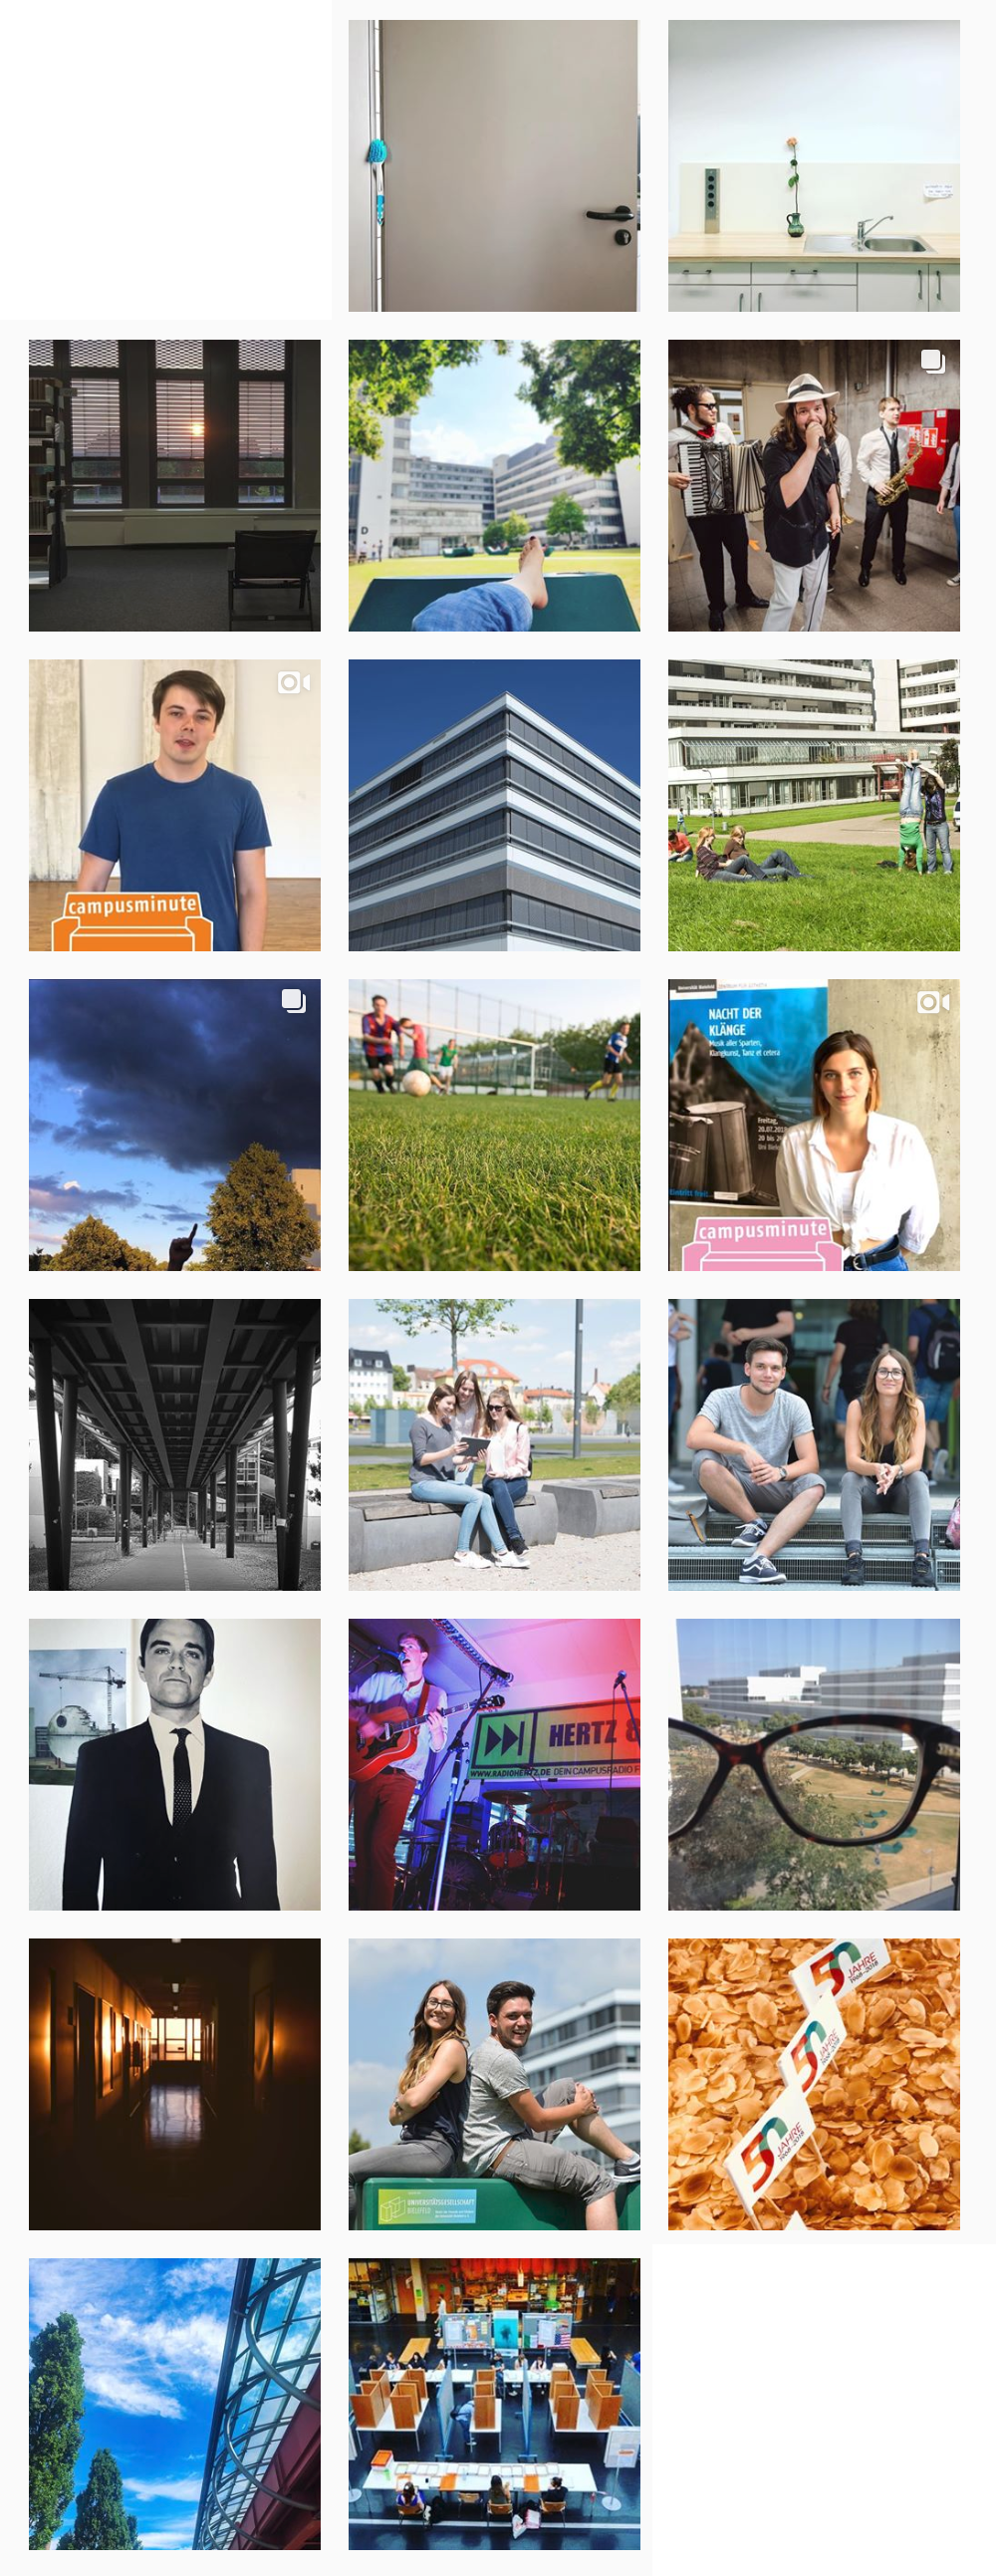
\includegraphics[width=0.6\textwidth]{img/posts/ig.png}}
    \caption{Instagram Posts - Universität Bielefeld - Juli 2018 \newline  \href{https://www.instagram.com/bielefelduniversity/}{instagram.com/bielefelduniversity}}
    \label{fig:socialmediapostsig}
\end{figure}

\begin{figure}[h]
    \centering
    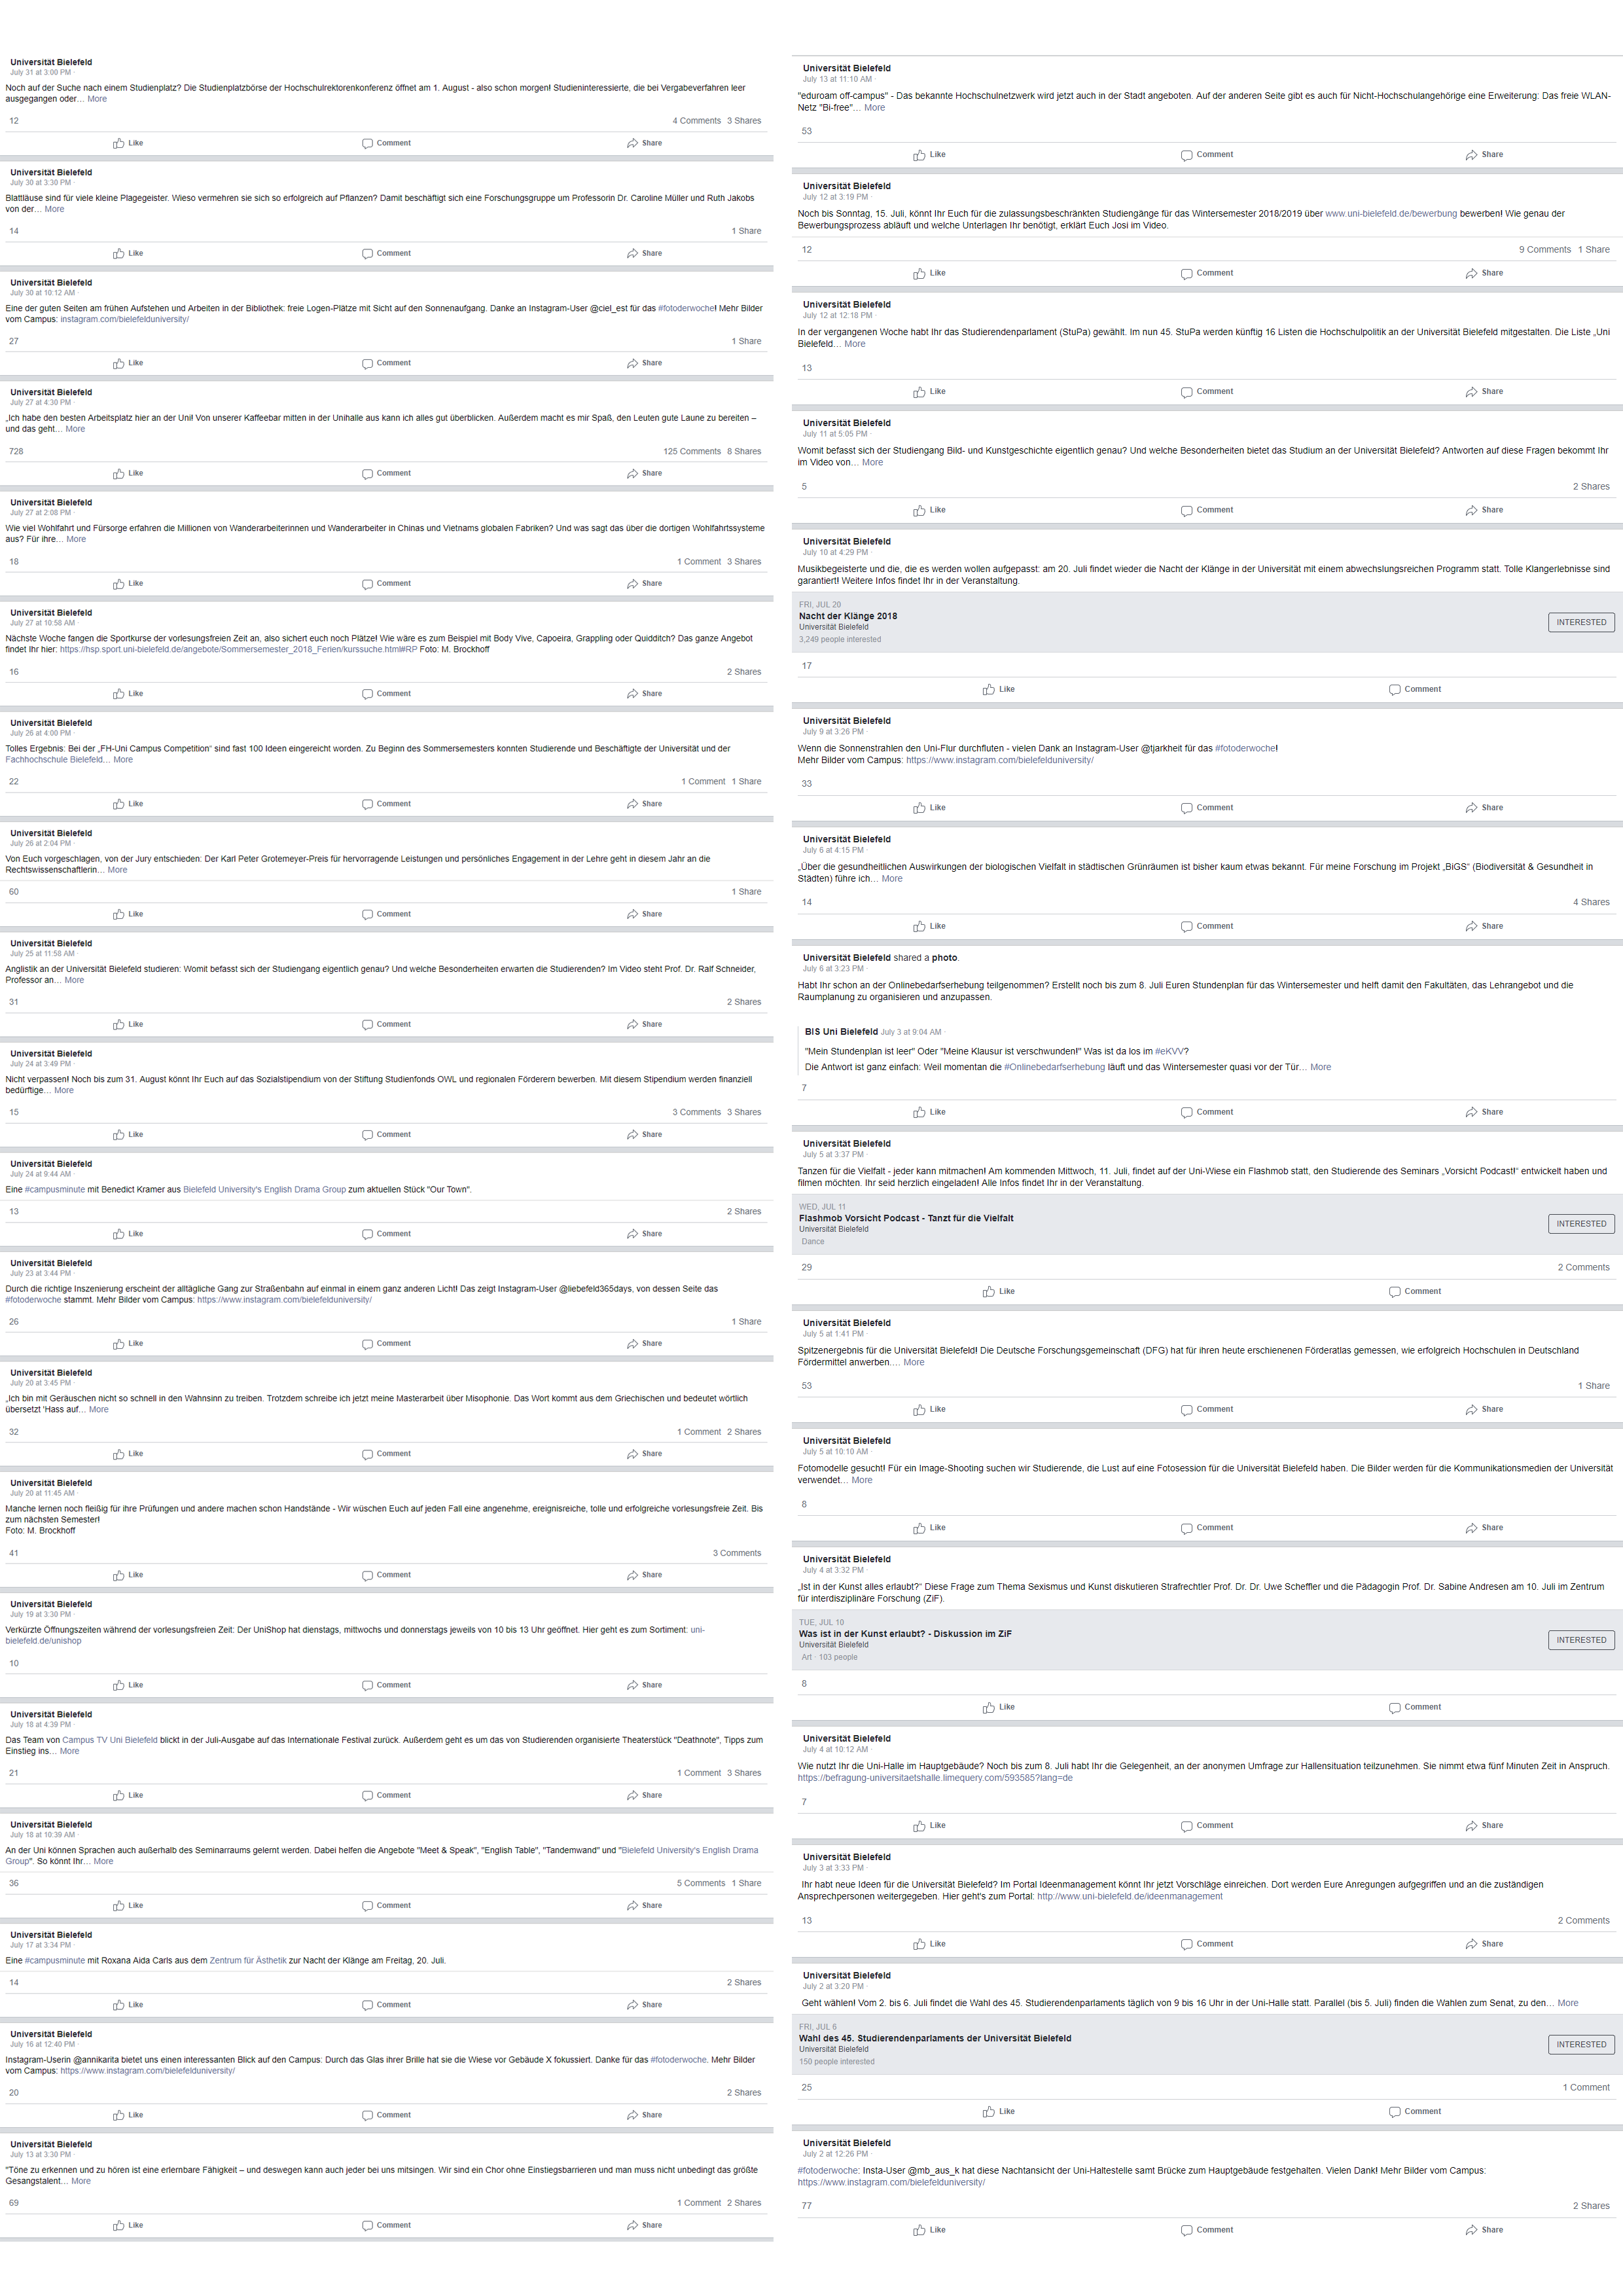
\includegraphics[width=1.2\textwidth]{img/posts/fb.png}}
    \caption{Facebook Posts - Universität Bielefeld - Juli 2018 \newline \href{http://www.facebook.com/bielefelduniversity}{facebook.com/bielefelduniversity}}
    \label{fig:socialmediapostsfb}
\end{figure}

\begin{figure}[h]
    \centering
    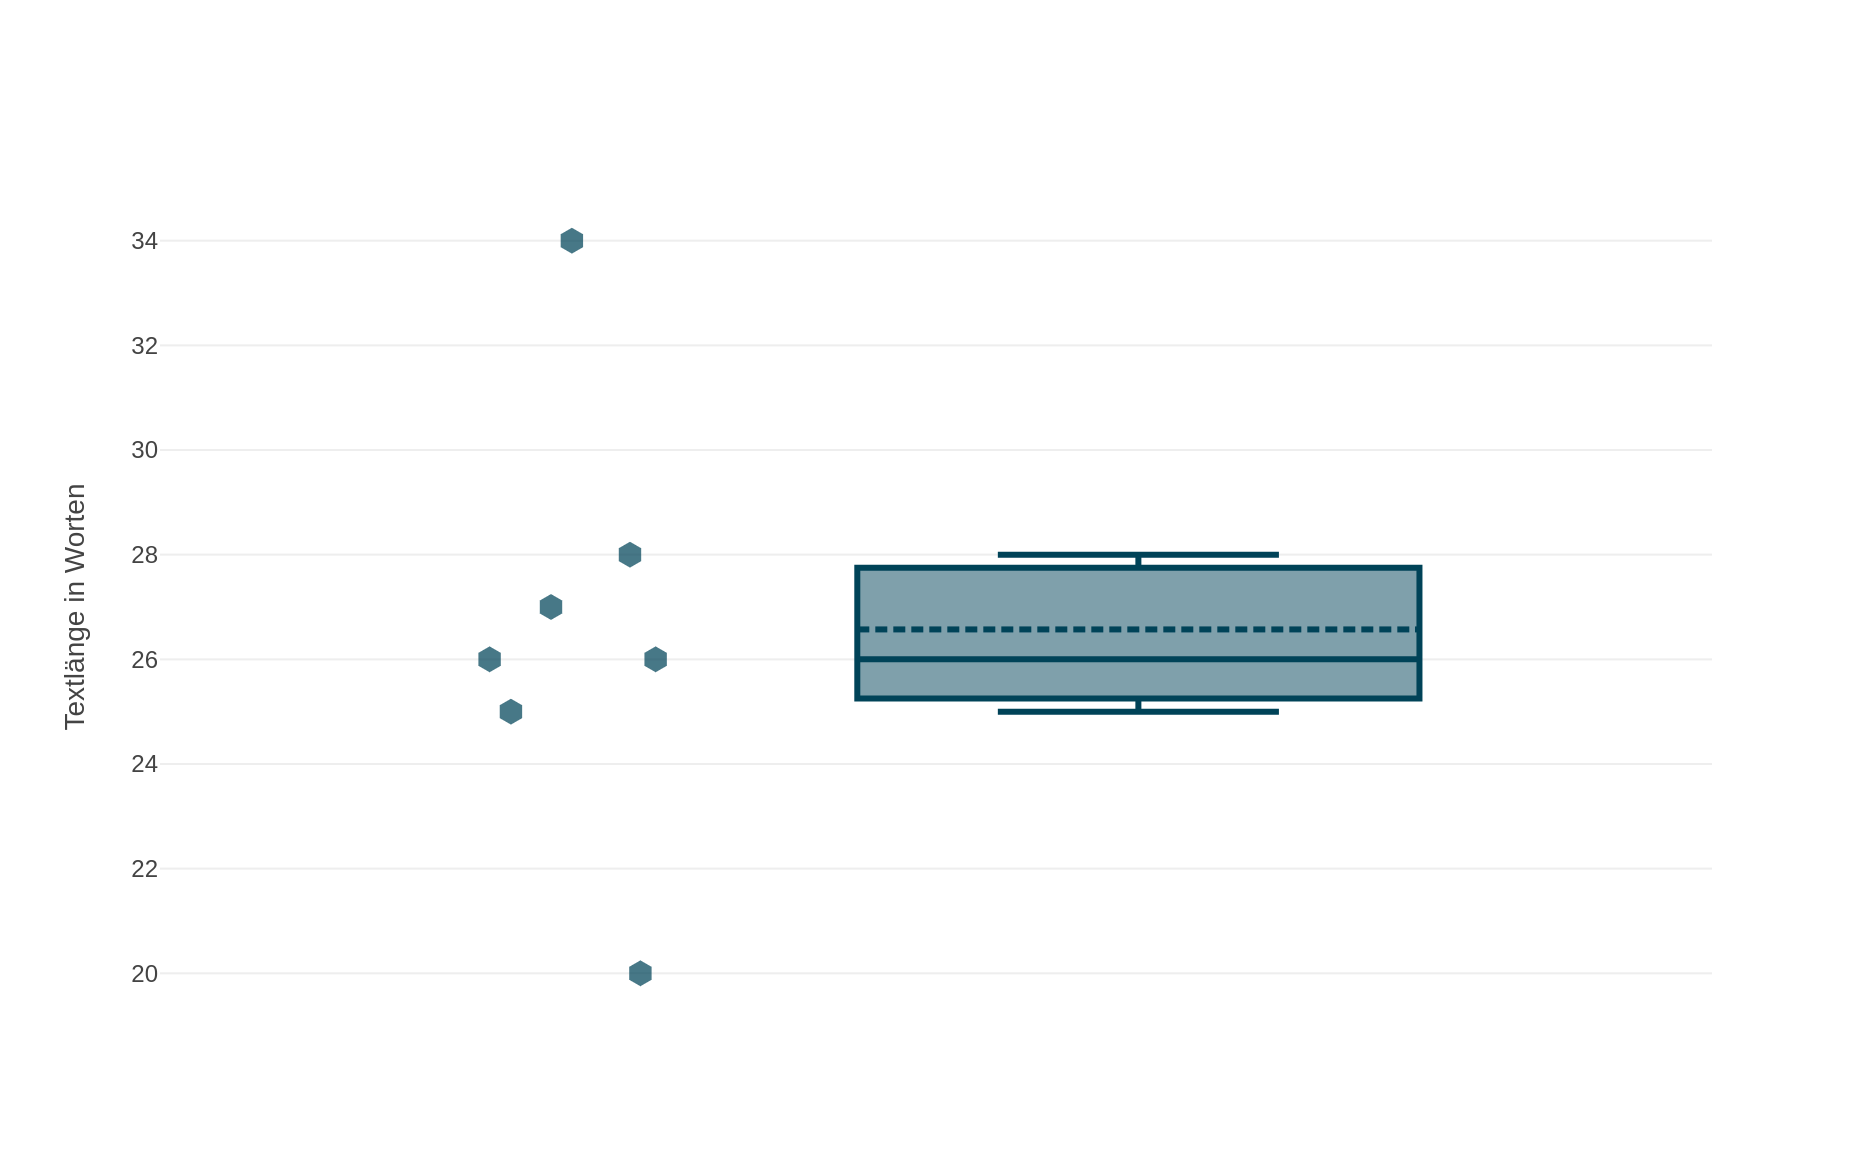
\includegraphics[width=1.2\textwidth]{img/posts/tw.png}}
    \caption{Twitter Posts - Universität Bielefeld - Juli 2018 \newline \href{https://www.twitter.com/unibielefeld}{twitter.com/unibielefeld}}
    \label{fig:socialmediapoststw}
\end{figure}

\begin{figure}[h]
    \centering
    \includegraphics[width=1.2\textwidth]{img/posts/bl.png}}
    \caption{Blog Posts - Universität Bielefeld - Juli 2018 \newline \href{http://ekvv.uni-bielefeld.de/blog/uninews/}{ekvv.uni-bielefeld.de/blog/uninews}}
    \label{fig:socialmediapostsbl}
\end{figure}



\end{document}
